%Template by Morten Espensen
%Deffinere kommandoer til om vores information

\documentclass[]{report}
%\usepackage{color}
%\usepackage{alltt}
\usepackage{amsmath}
\usepackage{amssymb}
\usepackage{float}
\usepackage[parfill]{parskip}
\usepackage{lscape}
\usepackage{enumerate}
\usepackage{amsmath}
\usepackage[danish,english]{babel}

\usepackage[paper=A4,pagesize]{typearea}
\usepackage[toc,page]{appendix}

\usepackage[utf8]{inputenc}
\usepackage{fancyhdr}
%\usepackage{boxproof}
%\usepackage{daymonthyear}
\usepackage{stmaryrd}

\usepackage{color}
\usepackage{fancyvrb}
\usepackage[usenames,dvipsnames]{xcolor}
\fvset{frame=single,framesep=1mm,fontfamily=courier,fontsize=\scriptsize,numbers=left,framerule=.3mm,numbersep=1mm,commandchars=\\\{\}}

\usepackage{wallpaper} % For the frontpage background

\usepackage{listings} % KODE SHIT
\lstset{ %
language=PHP,          		    % the language of the code
basicstyle=\footnotesize,       % the size of the fonts that are used for the code
numbers=left,                   % where to put the line-numbers
numberstyle=\footnotesize,      % the size of the fonts that are used for the line-numbers
stepnumber=1,                   % the step between two line-numbers. If it's 1, each line
                                % will be numbered
numbersep=5pt,                  % how far the line-numbers are from the code
backgroundcolor=\color{white},  % choose the background color. You must add \usepackage{color}
showspaces=false,               % show spaces adding particular underscores
showstringspaces=false,         % underline spaces within strings
showtabs=false,                 % show tabs within strings adding particular underscores
frame=single,                   % adds a frame around the code
tabsize=2,                      % sets default tabsize to 2 spaces
captionpos=b,                   % sets the caption-position to bottom
breaklines=true,                % sets automatic line breaking
breakatwhitespace=false,        % sets if automatic breaks should only happen at whitespace
title=\lstname,                 % show the filename of files included with \lstinputlisting;
                                % also try caption instead of title
escapeinside={\%*}{*)},         % if you want to add a comment within your code
morekeywords={*,...,xchar,xstring,xmany1,chainl1,chainl1',ReadP}            % if you want to add more keywords to the set
}

\newcommand{\theassingment}{Development of E-learning concept\\[1.6ex] \hspace*{-2.39cm} for Medical Doctors}
\newcommand{\thesubassignment}{Design Project Report}
\newcommand{\shorttheassingment}{ITIaC}
%\newcommand{\thepaperauthor}{}
\newcommand{\personalid}{dzr440 - 19/06/1991}
\newcommand{\thesubject}{IT Innovation and Change}
\newcommand{\theinstitute}{Department of Computer Science}
\newcommand{\thesupervisor}{Cosmin E. Oancea} %behøves kun hvis findes

\newcommand*{\diffdchar}{\mathrm{d}}    % or {ⅆ}, or {\mathrm{d}}, or whatever standard you’d like to adhere to
\newcommand*{\dd}{\mathop{\diffdchar\!}}

\newenvironment{timesfont}{\fontfamily{mathptmx}\selectfont}{}

\setlength\parskip{2ex}
\newcommand{\n}[0]{\\[2ex]} %NEWLINE [2ex]
\newcommand{\set}[1]{\{#1\}}
\usepackage{hyperref}

\newcommand{\fnurl}[2]{\href{#2}{#1}\footnote{\url{#2}}}  %foodnote url ref \fnurl{String}{Link}

\newcommand{\premise}{\=\mbox{premise}}
\newcommand{\assumption}{\=\mbox{assumption}}
\newcommand{\landi}{\=\intro\land : }
\newcommand{\lande}{\=\elim\land_{1} : }
\newcommand{\landee}{\=\elim\land_{2} : }
\newcommand{\lori}{\=\intro\lor_{1} : }
\newcommand{\lorii}{\=\intro\lor_{2} : }
\newcommand{\lore}{\=\elim\lor : }
\newcommand{\toi}{\=\intro\to : }
\newcommand{\toe}{\=\elim\to : }
\newcommand{\lnoti}{\=\intro\lnot : }
\newcommand{\lnote}{\=\elim\lnot : }
\newcommand{\bote}{\=\elim\bot : }
\newcommand{\lnege}{\=\lnot\elim\lnot : }
\newcommand{\lnegi}{\=\lnot\intro\lnot : }
\newcommand{\leqi}{\= \intro= }
\newcommand{\leqe}{\= \elim= : }
\newcommand{\lforalli}{\= \intro\forall : }
\newcommand{\lforalle}{\= \elim\forall : }
\newcommand{\lexistsi}{\= \intro\exists : }
\newcommand{\lexistse}{\= \elim\exists : }
\newcommand{\MT}{\=MT : }
\newcommand{\PBC}{\=PBC : }
\newcommand{\LEM}{\=LEM : }

\newenvironment{changemargin}[1]{
  \begin{list}{}{
    \setlength{\voffset}{#1}
  }
  \item[]}{\end{list}}


\usepackage{hyperref}
\usepackage{pdfpages} % til at tilføje apendix
\usepackage{graphicx}
\DeclareGraphicsExtensions{.pdf,.png,.jpg}
%\usepackage[backend=bibtex]{biblatex} %backend tells biblatex what you will be using to process the bibliography file
%\bibliography{report.bib}
\def\thesection{\thechapter.\arabic{section}}
%\renewcommand{\thesubsection} {\thesection.\alph{subsection}}

\pagestyle{fancy}
\fancyhead{}
\fancyhead[LO,LE]{\shorttheassingment}
\fancyhead[RO,RE]{\today}
\fancyhead[CO,CE]{\theinstitute}

\setcounter{secnumdepth}{0}
\setcounter{tocdepth}{3}

\begin{document}
\begin{titlepage}
\begin{timesfont}
% Import the ku frontpage graphics
\ThisULCornerWallPaper{1}{nat-farve.pdf}
% Import faculty title
\ThisULCornerWallPaper{1}{nat-en.pdf}
% For forklaring af vspace og stretch, se side 115 i ".. not so short .."
% www.ctan.org/tex-archive/info/lshort/english/lshort.pdf
\vspace*{3cm}
\hspace*{-2.3cm}
% Her vælger en kæmpe skrifttype og fed skrift
\Huge\bfseries
\vspace*{-0.5cm}
\theassingment\n
\hspace*{-2.4cm}
-- \thesubassignment \n
\LARGE
\hspace*{-2.4cm}
\vspace*{-0.5cm}
\thesubject \\[2.2ex]
\hspace*{-2.4cm}
\vspace*{5.0cm}
\theinstitute \n
\hspace*{-2.38cm}
\large
\textbf{Written by:}\\[1ex]
\hspace*{-2.33cm}
Morten Espensen (dzr440)\\
\hspace*{-2.33cm}
David B. Gandrup (vpd177)\\
\hspace*{-2.33cm}
Sokratis S. Drosos (dnb823)\\
\hspace*{-2.33cm}
Bjarki Madsen (lch929)\\
\hspace*{-2.33cm}
Niklas Høj (nwv762)\\
%\vspace*{1cm}
\hspace*{-2.33cm}
% Nulstiller skriftstørrelse og type (f.eks. fed)
\normalsize
% VEJLEDER INFORMATION I PÅ FORSIDEN?
%\thesubject \n

\hspace*{-2.33cm}
%\textbf{\emph{Supervised by:}}

\hspace*{-2.33cm}
%\thesupervisor

\end{timesfont}
\end{titlepage}
\tableofcontents



\newpage
\abstract{Doctors are mostly overly busy individuals with strict schedules. Engaging them with available learning material via digital platforms therefore requires a finely tuned approach that is able to catch the doctor in an available state where they are willing to discover opportunities to evolve their continuous professional development (CPD). In this report, we use the MUST method, a participatory design method that introduces innovative change to an organisation, to design and recommend a solution for the Danish Medical Association (DMA). In particular, we introduce our own method called Hook and Reel which tries to engage doctors in the smallest time-frame available (the hook) and have them discovering and using the material (the reel). We describe in detail the methods used that lead us to our findings, our coherent visions of change along with the illustrative prototypes that put our visions in a context of the existing systems found in DMA’s domain. }
\section{Summary}

\subsection{The Problem}
The Danish Medical Association (DMA) currently has a large amount of courses, online and not, accessible to their members, both free of charge and paid for. The courses’ topics are also widely ranging from informing doctors of new medical treatments to development on their own personal skills. In spite of this, DMA sees very little usage of its available material, especially from the older generation of doctors where their feedback indicates that it is a “break from responsibility” to use the existing continuous education system whilst working. This indicates that time does play a large factor here, since the courses require an allocated time in the doctor’s daily work routine, and sometimes requires entire days being taken out of their schedules to attend courses. Having finished a course, the doctor can add the newly acquired skills to his/her CV but not much more, which also raises the concern of a lack in motivation for taking the courses to begin with. For example, the British Medical Association (BMA) encourages their members to build up their e-portfolio by finishing courses that \fnurl{give credits for their continuous professional development (CPD)}{http://bma.org.uk/developing-your-career/career-progression}, but we have nothing like that in Denmark where each doctor is simply expected to maintain their own continuous education.

The DMA has a lot of data on the usage of their website which show that doctors do visit the learning part of the website, but generally spend very little time there. On average they spend a few minutes, which is far less than the necessary time required to complete a course or in many cases even sign up for one in the first place. Additionally, the traffic to the website mainly comes from desktop computers, but traffic from mobile devices is steadily increasing, although the current learning platform is not optimised for them.

Even though there might be allocated time in doctors’ work schedules, there is not much of an incentive to take courses beyond an obligation to do so, and keeping up with new knowledge might in the end just become a hassle as taking away precious office hours which some doctors think are better spent practicing medicine.

\subsection{In this report}
This report consists of our visions of overall change. In it we propose and suggest innovative changes to DMA’s organization as well as changes to the usage of current available systems in DMA’s domain. We base these changes on the results of the four phases of the MUST method \cite{bodker} i.e the Initiation phase; In-line analysis phase; In-depth analysis phase and finally the Innovation phase. Figure \ref{fig:baseline_plan} shows these four phases and our documented activities within each one.

\begin{figure*}[h!]
 \begin{center}
  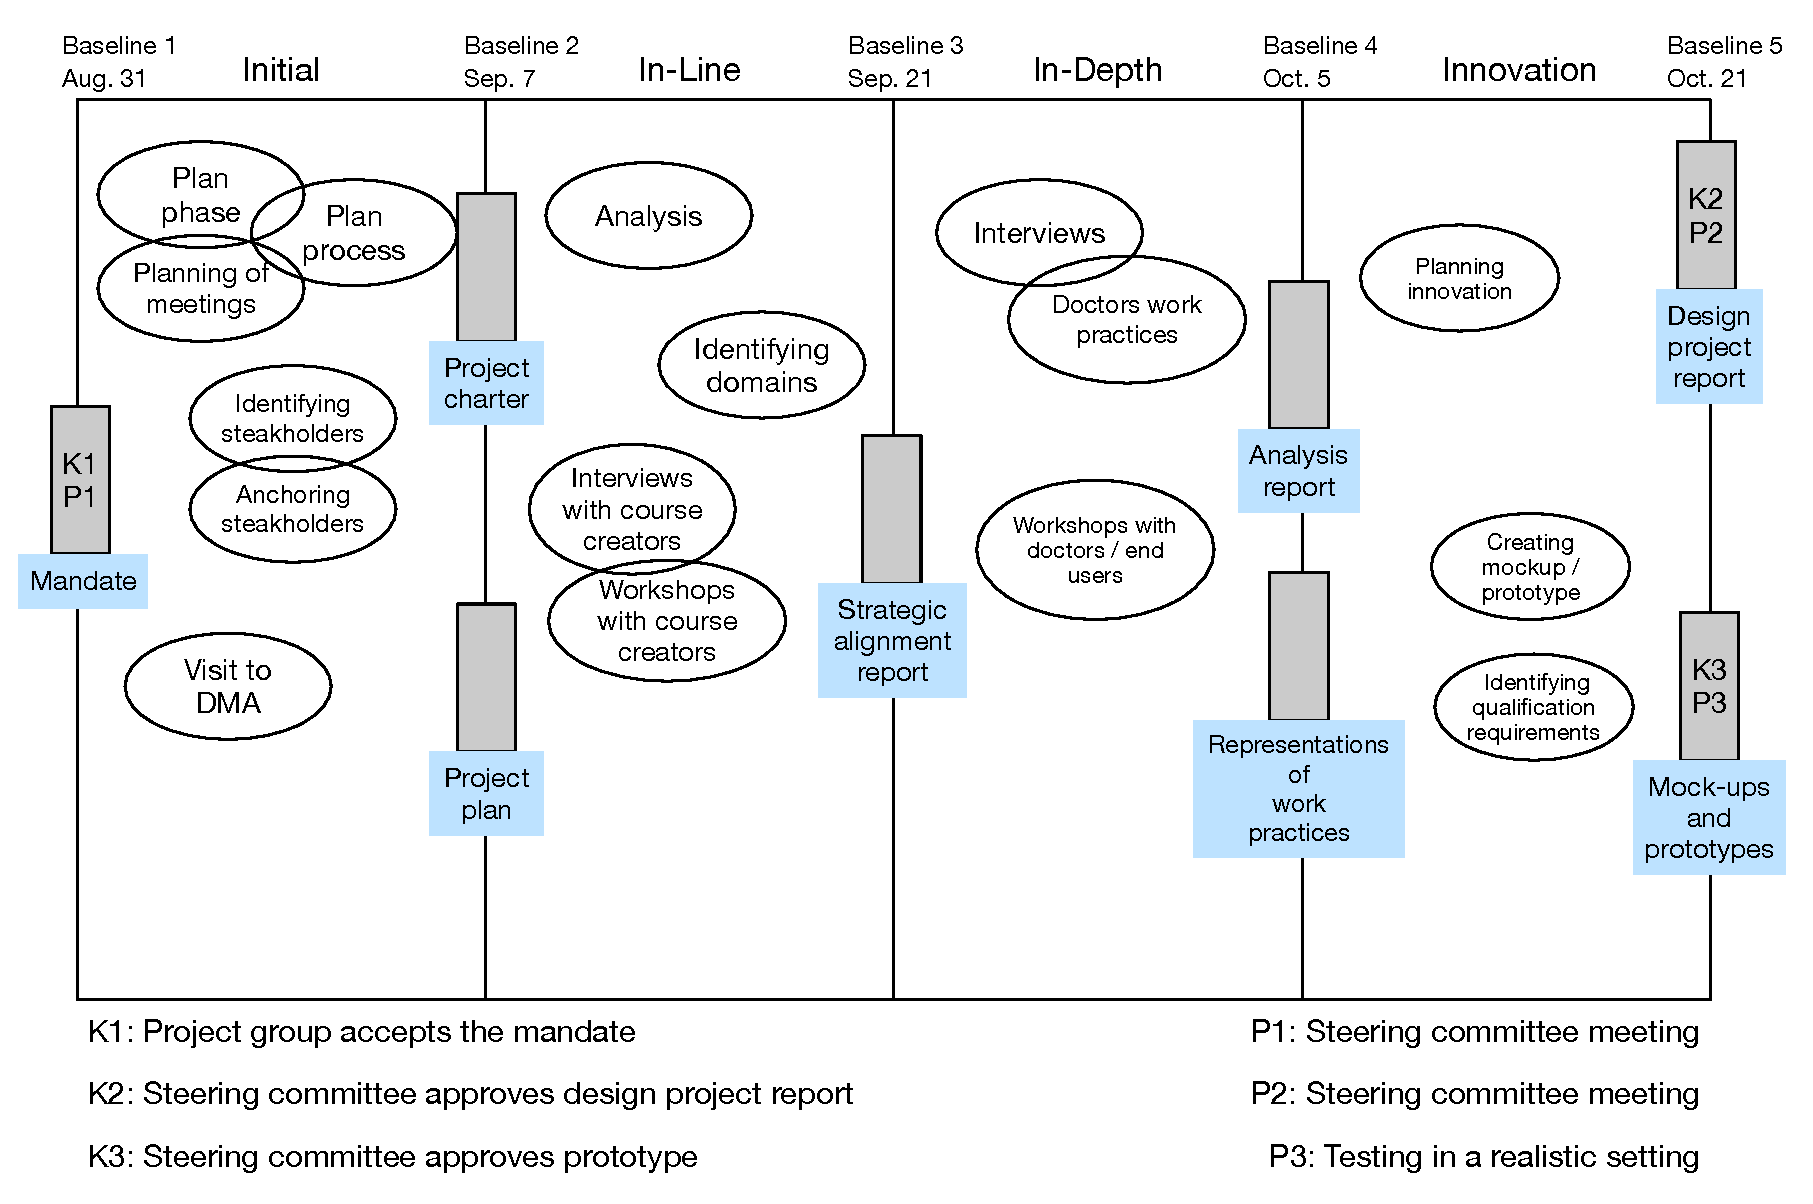
\includegraphics[width=1\textwidth]{figures/baseline-plan.pdf}
  \caption{Our baseline-plan for the project.\label{fig:baseline_plan}}
 \end{center}
\end{figure*}



Given the high complexity of the general problem and our time limitations, we decided to focus the scope of the innovation to something very specific, in this case, the doctors’ time. We have therefore attempted to come up with ideas on how to engage them in a very limited timeframe. This is opposed to coming up with ideas that target completely new platforms for e-learning or making up ideas about how the course material should be presented for doctors (i.e divide courses into multiples of smaller segments).

Our proposed solutions are based on the assumption that doctors are overly busy individuals that have to be engaged with a well defined approach using methods that we like to call Hook and Reel. Hooks can come in different formats, e.g a video, a test or an image, but they all share the same purpose, to hook the doctors and reel them in a very short timeframe.

This report is structured as follows. Section \textit{Methods} on page~\pageref{sec:method}. Section \textit{Objective} on page \pageref{sec:objective} goes through the main points and results of the first three MUST phases. Section \textit{Vision of overall change} on page \pageref{sec:vision} goes into detail of our visions of the overall change, where we identify changes to the technology, DMA’s work organization and required qualifications to implement said changes. Section \textit{Advantages and disadvantages} on page \pageref{sec:advantages} is about the advantages of our proposed solution with regards to DMA’s business strategy. Section \textit{Finances} on page \pageref{sec:finances} talks about the cost of implementation. Section \textit{Implementation strategy and plan} on page \pageref{sec:implementation} introduces our recommended plan to implement our visions of change with regards to technicality and organization. Finally, section \textit{Recommendations and priorities} on page \pageref{sec:recommendations} includes final words on additional recommendations and priorities for DMA.


\section{Method}


<<<<<<< HEAD
In this section we will discuss some methodological concepts that we find especially interesting in relation to our project and which we think have had a direct impact on the end result. 

\subsection{Problematisation}
As we started the project with DMA, the general idea was about implementing an e-learning platform to help facilitate the learning experience of its members. However, as we moved through the MUST method and as we finished the in-line analysis, we realised that this was not possible, due to the lack of genuine user participation\cite{bodker} and the limited amount of users, that were willing to participate in the project. 

Once we analysed the Environment, Business and IT Strategies and the Work domains \cite{bodker}, it was clear that we would not be able to propose an innovative idea about a new e-learning platform but rather propose ideas based on the existing ones. 

Through the Innovative Technology Analysis\cite{bodker}, we examined how new technological potentials can impact or alter the business strategy. This was done by performing interviews with the employees involved in the potential uses of IT. However, we were not able to get any documents concerning the existing IT system description or the one currently being developed and we were limited to performing a SWOT analysis.

As a result, the outcome of the in-line analysis phase, which also includes a problematisation of the premise for the entire design project, shifted towards a more technically general approach. This approach consisted of using the existing emailing platform of DMA, in order to attract more members into using the provided e-learning solution by DMA.


\subsection{Spokespersons}
In our project there has been quiet few spokespersons involved. This was caused by first of all our big focus on problematisation combined with the short timeframe in which this project was executed. The main spokespersons during our project were:

\begin{itemize}
\item Lene Rybner - DMA
\item Birgitte Rode Diness - Rigshospitalet
\item Claus Arwilk - DMA
\end{itemize}


Among these spokespersons only Lene was the only person participating in our steering committee and was a representative of DMA. Lene also had great responsibility in the project as she was partly responsible for helping us reaching out to possible spokespersons in the medical field and creating interessement, in order to lock these in, as discussed in\cite{callon}. Birgitte was representative of course creators in the medical field as she had created a blended learning course and had contact with DMA. Claus representative of the IT development team at DMA who would potentially be responsible of implementing the ideas.

During our project we had attempted to reach out to several doctors, who would be representative of different kinds of doctors. As we in our project greatly needed to create interessement and have people become spokespersons for the different roles. This became a real issue as we had to rely on Lene as our contact to DMA to help us with creating the interessement and contact to doctors who fit the different audiences such as course creators, course participants and so forth.

<<<<<<< HEAD
Ultimately, we were so time constrained that when we finally got contact to a group of people who had attended Birgittes blended course we felt that our only option in order to actually utilise this contact to hear and use their opinion was to send out a questionnaire to have them represent the role of course attendant, as discussed in Section \ref{indepth-approach}
=======
Ultimately, we were so time constrained that when we finally got contact to a group of people who had attended Birgittes blended course we felt that our only option in order to actually utilise this contact to hear and use their opinion was to send out a questionnaire to have them represent the role of course attendant, as discussed in the course participants section on page \pageref{indepth:questionnaire}.
>>>>>>> 7c5c6f0cb53d363ea36fe6ac624f50815a9109c2

We also spoke to another doctor, Jacob Melchiors, from Rigshospitalet, who would have been a great representative of the course participants. He would also have liked to assist us in our project and possibly participate in our steering committee. But this was rather late in our project and was mainly based upon his interest in learning methods and e-learning solutions. At that time we were already at a point, where we were just about to present our idea for our steering committee, Lene, and thus no longer considering designing a e-learning platform in reality, but instead move to the mandated idea of our project, where we would develop ideas to promote existing course material.

Having established contact this late meant that we had no time to meet with Jacob prior to obtaining the mandate for our direction, at which point we felt it would be pointless to include him in our steering committee as he would not have a lot of influence afterwards. Thus, in order to not waste his time without giving him influence we chose to stay with our current project construction. This was unfortunate as we had been looking for a representative such as Jacob, as he was able to represent the target audience which DMA had in mind in their case description.

The case with Jacob along with Birgittes course participators where we had to make an number of time sensitive decisions which likely greatly impact our project as discussed in \cite{key-to-success-p1}, where as in a utopian world we would have preferred to expand our steering committee in order to include representatives of each of the affected roles as suggested in \cite{callon}, which we somewhat lacked in our project. Thus having had a few course creators and course attendees, possibly in different age groups, as participants could possibly have changed the direction of our project entirely.

Accordingly more involvement or data from the IT development team might also have proven fertile, as we believe integration of any innovation is essential to its success in cases such as ours where users want to access the content we are trying to provide in a simple and streamlined way. Unfortunately this was not really possible given the issues described in the implementation section on page~\pageref{sec:implementation}. This might have been less of a problem if we had person from IT in our steering committee, such that this person could participate in the design of our innovation.

\section{Objective}
\subsection{Objective and Premise of the Design Project }
The design project is based on the case as presented by DMA entitled “Digital One-Day Courses for Doctors” <Reference to the case description as an appendix?>. The direct goal of the case description is the development of a “digital learning platform”. The motivation is to provide to the more than 27000 members (per January 1. 2014) more courses on demand and give them an overview of available online courses both nationally and internationally.

The DMA had a focus group develop requirements for the platform and easy access triumphed over variety, looks and features as the most important consideration. Additionally, the case asks us to consider the following:

\begin{enumerate}[A.]
\item Will there be in a foreseeable future sufficient demand for digital learning services and/or platform from DMA members?
\item What do the end users require from a digital learning platform?
\item How can a digital learning platform be implemented within the existing organisation of DMA?
\item What is the ‘minimal viable product’ i.e. the most simple inexpensive product that allows DMA to enter this market?
\end{enumerate}

And in the pursuit of these to explore:

\begin{itemize}
\item What are the reasons for the current lack of incitement for the digital offers?
\item How can digital learning  be embedded in the daily work of doctors, who typically demand a decent work-life balance, and who typically prefer education to be something that happens in a formal setting such as a course or conference?
\item Is it more suitable continuing the current ad-hoc strategy, or does the increased uptake of digital learning offer a more holistic, top-down strategy and thus also a platform?
\item What devices will best support the learning situation: Computers, tablets or smart phones, or should the solution be compatible with all types of devices?
\end{itemize}

DMAs expectations to the solution were:

\begin{itemize}
\item A specification of a strategy that will provide the members of the DMA with more digital learning possibilities. This includes considerations about the cost structure, resource requirements etc.
\item A specification of the user requirements and design of a digital learning service offers that sufficiently fit with the existing organisation in DMA.
\item A design proposal for the learning service, including considerations regarding distribution of this.
\item A specification of the overall technical requirements for such a solution, including recommendations for the software platform, and considerations regarding integration with the existing web page www.laeger.dk.
\item Considerations regarding channels for distribution of the service (e.g. via the existing homepage or via app stores).
\end{itemize}

We had some ideas to what might fulfil the noted requirements as we started the project. The main idea we discussed was an e-learning platform where courses were “chopped up” into 5 minute bits that would be easy for the doctors to fit in and follow in their busy schedules.

In the initial phase of the MUST method, our approach was to establish a thorough understanding of the organisational setup of DMA and identify the main stakeholders. This allowed us to understand the scope of the project and eliminate all potential misunderstandings between the project group and the steering committee. In the first meeting with the steering committee , which consisted of Lene Rybner as the sole member, we got to know the project better and what the wishes and expectations of DMA were.

Based on our understanding and expectations at the time, we made a baseline plan for the project <Figure reference, insert figure below>\footnote{TODO: FIX THIS}. The deadlines and outcome of each phase of the project was dictated by the course structure, so this was unchanged, but we later made an updated baseline plan <Figure reference>\footnote{TODO: FIX THIS} that describes the actual activities in each phase.


\section{In-line Analysis Phase}
\subsection{Approach}
Our approach in the in-line analysis phase was to, firstly, figure out the major work domains to get a sense of where the IT system was used and where innovation could actually be required, and secondly, dig a little deeper into DMA’s organization by discovering some of their business strategies behind course creation, how are they created, who provides them and what are the main platforms of the courses.

\subsection{Environment}

The Danish Medical Association (DMA), Lægeforeningen in Danish, is an association that aims to represent all Danish doctors and their associated organisations such as unions, tying them all together and providing benefits for all its members. There are three major medical organisations under the DMA. The structure is illustrated in figure \ref{fig:dmaorganisation}.

The first is “Yngre Læger” (YL), an association for younger doctors with close ties to doctors advancing their studies in the “klinisk basisuddannelse” (KBU), those taking their introduction to their speciality and those who are actively specialising.

The second is “Forening af Speciallæger” (FAS) which is a union for consulting doctors that have studied a speciality.

Lastly is “Praktiserende Lægers Organisation” (PLO) which is an organisation for the practicing family doctors, who usually run their own local clinic for the nearby population.

Danish doctors are generally associated with one of these three organisations and are thus members of the DMA, having access to the DMA provided courses and other benefits.

\begin{figure*}[h!]
 \begin{center}
  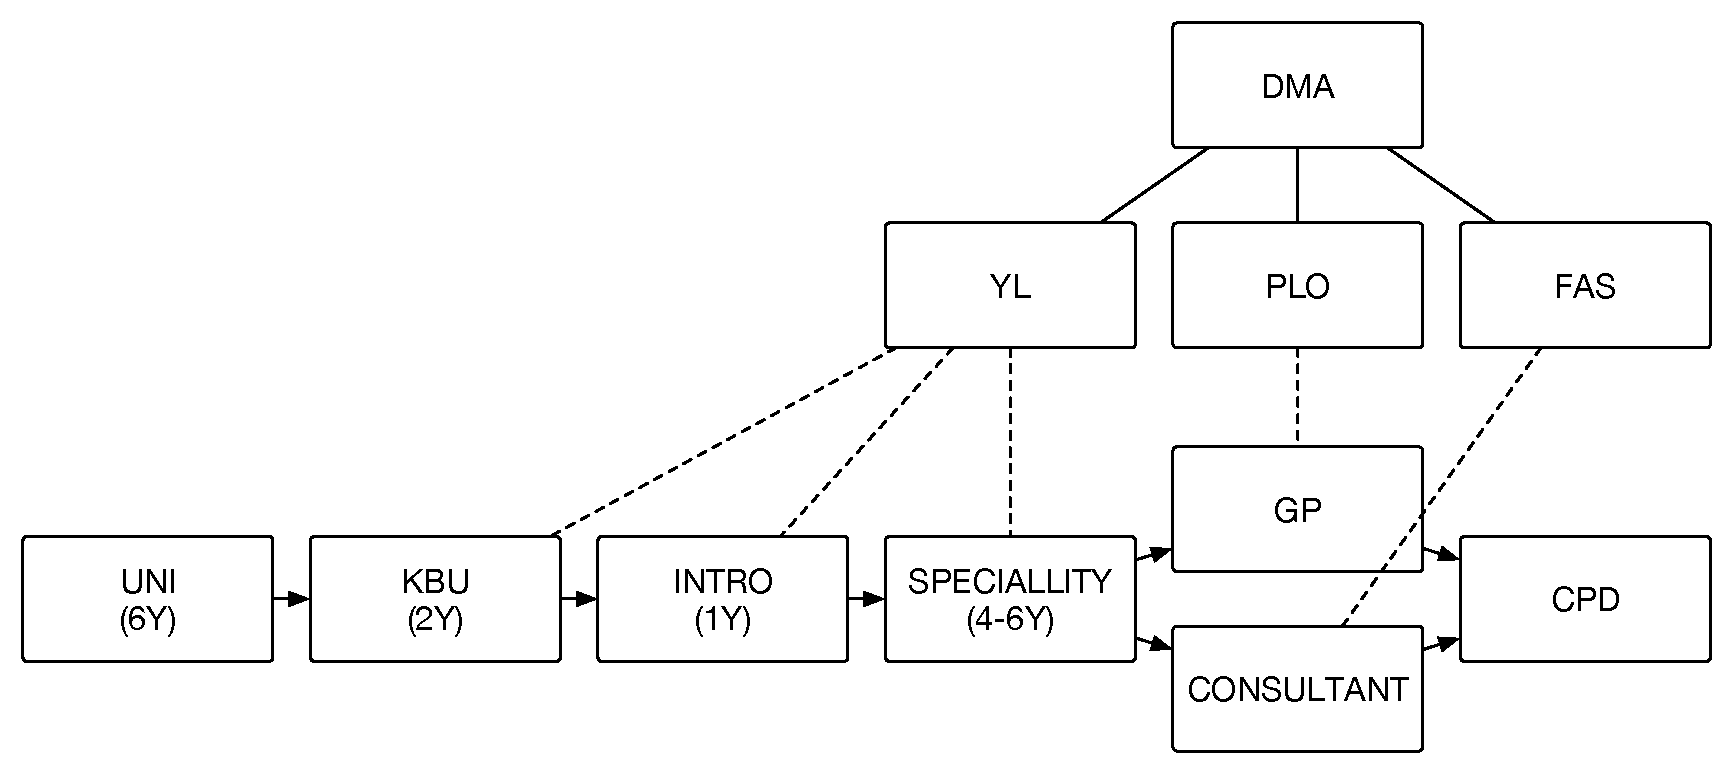
\includegraphics[width=1\textwidth]{figures/dma-structure.pdf}
  \caption{The organisation of DMA.\label{fig:dmaorganisation}}
 \end{center}
\end{figure*}

\subsubsection{Potential and Needs}
DMA members need to take courses in order to stay up to date with the latest information about medicine practices. So far the existing e-learning platforms that provide the necessary courses are not widely used by the doctors, in some cases this is because they consider it to be time consuming. Some doctors also consider the contents of the e-learning courses to be too easy and superficial <Reference?>. What is needed is a new way to deliver information to the doctors, such that we can engage them in a way that eliminates the concerns of the current e-learning solutions.


\subsubsection{Requirements and Conditions}
DMA members are looking for a new e-learning platform with a different approach compared to the existing offers provided by DMA, such as BMJ Learning, since the DMA members do not currently utilise the offers as much as expected. DMA would like to have the content focused on including the entire spectrum (known as the 7 roles of physicians) of knowledge areas, which a modern doctor should be educated in, for example there should be topics dealing with communication, administration and so on. Currently surveys performed by DMA show that some doctors prefer to strictly focus their education on medical expertise and entirely neglecting being educated in the remaining 6 roles.

\subsubsection{Business Strategy}
\begin{description}
\item[Goals:] We aim to find an approach for busy doctors to learn course material that will work for them. The approach should be realistic and feasible within the constraints of the target association DMA, and should actually engage the doctors and fit their needs such that the doctors will use it in practice.
\item[Business Processes:] We did not consider business processes very relevant in this phase of the project. DMA has a dominant market position with 98\% of Danish doctors being members and a fixed membership fee subscription model, which was something we learned later.

We do not consider business processes relevant at this time, as it is outside the scope of our study.
\item[Challenges and Problems:] There are various challenges associated with solving the problem of doctors not actively continuing their education despite attempts to facilitate their learning. Firstly, we had to establish what was actually causing the problem. The cause seems to be that the doctors do not have time in their busy schedules to take hours or entire days off to study and take courses, but is this actually the main cause? Is there more to it? Are other factors in the way of doctors keeping up with their fields?

If the stated problem is confirmed to be what it seems to be, then we still have the problem of figuring out an alternative method of providing the course materials in a manner that is accessible to the doctors. And even with accessible learning, the approach still needs to motivate the doctors to actually use the solution. So we need to understand exactly what the doctors are looking for in a way of consuming courses and what exactly will suit their needs.
\end{description}

\subsection{Work Domains}
We have identified two primary work domains: Course creation and Doctors practice.

\textbf{Course Creation}
\begin{description}
\item[Definition:] The course creation work domain is the source that DMA uses to provide material for their members to educate themselves. It is not limited to the creators that DMA is directly linked with, but also external third party creators.

\item[Characterization:] DMA has multiple sources of courses and material of differing types and they are delivered in different ways, from BMJ’s e-learning platform, DMA’s own courses and courses created elsewhere and communicated to members through and by DMA.
The sources have different delivery methods, course content, evaluation methods and purpose.

DMA primarily uses their website and other IT based channels to inform their members of the existence of these courses, and to some extent also give access to them, for example by providing discounted membership fees to BMJ’s e-learning platform.
\item[Discussion/Conclusion:] The constraints and methods in course creation are key to determining what is possible to actually do in terms of innovative ideas.

\end{description}

\textbf{Doctors Practice}
\begin{description}
\item[Definition:] The actual work practice and daily schedule of DMA’s members, the doctors, and how much time and resources they have available for learning new things. This means both considering the day to day work schedule and any time dedicated to learning.

\item[Characterization:] Although DMA serves a very diverse member group, there is some common ground and work practices among a large part of their members. The doctors have a busy working day that is not very flexible, making it difficult for them to make time for the current format of provided courses.

Additionally some members lack incentive to prioritise learning over working, as some doctors are paid to learn, others are not.

\item[Discussion/Conclusion:] Whatever the quality of the courses provided by DMA may be, the doctors have to be able to find the time to take them. The courses also need to cater for the actual interests of the doctors and be relevant in their daily work.


\end{description}


\section{In-depth Analysis Phase}
\subsection{Approach}
Based on the results of the in-line analysis phase we interviewed a doctor who was also a course creator, sent out a questionnaire to a range of doctors and interviewed our key spokesperson at DMA, Lene Rybner. We intended to do work practice observations of doctors, but this proved too difficult to set up and we abandoned this in favor of the questionnaires and further interviews with Lene.

\subsection{Work Practices}
From an interview with a person who is both a doctor and a course creator of CPD material the project group was able to identify work practices at both ends of the table and help view the project from two different points of views.

We started asking her questions with regards to her role as a course creator. She had helped creating and managing a course on genetics, which she ran as an introductory course to raise awareness of genetics being a fully fledged medical field. The online platform chosen for the course was itslearning where all course material, exams and discussions were kept. This course had previously failed to start twice due to lack of participants.
Once they started using the DMA’s monthly email newsletter instead of a system that required a login (itslearning) to post the information about the course, they gathered enough participants.

We then switched question topics and started asking her questions with regards to her role as a doctor. When we asked if she would have 5 or 10 minutes of spare time at some point in her schedule, if she could see herself taking a fragment of an e-learning course, her answer was that the material would have to be very accessible. She has signed up for BMJ before but the slightest resistance such as a complicated login to a different system kills the “will to learn” moment.

The email newsletter is therefore a critical channel in engaging doctors and it makes good sense based on their current work practices. The email does not require a complicated login and it is right there in front of them when the doctor uses his/her computer. Doctors are usually too busy with other things on their mind than logins to different systems, so the accessibility to the course material is a critical point as well.

Throughout our interviews with Lene, we discovered that she is the one responsible for making the available courses or material known to the doctors’ community. She has created various accounts on social networks (Facebook, LinkedIn), through which she promotes various courses that are available on DMA, BMJ, MOOCs and other e-learning platforms. In our last meeting we discussed about what would be the preferable time limit for an online course, we suggested a 7 minute time limit  and she replied that it is too much for the doctors to spend that amount of time.

In order to suggest various courses to the doctors she has to search through the courses herself in the above mentioned sites and post them on Facebook groups and various home pages that doctors visit. Lately she has started posting pictures concerning medical problems that are not “graphic” as she stated, but interesting enough to make the doctors look up the courses she suggests. However, she has no way of knowing if her methods work, because everything is hosted in websites that are not hosted by DMA (Facebook, LinkedIn), hence she cannot have any information about the traffic.

\subsection{Course Participants}
In addition to the interviews we also sent out a questionnaire. We would have liked to interview many more people, but due to limited resources this was not feasible, and so a questionnaire provided a good means of looking into the needs of a group of actual doctors in the DMA. The group of DMA doctors we had access to were those who had participated in the Genetics Course provided by the DMA, which we were also given access to in our case study. Of these, 6 participants consented to participating in our questionnaire. However, at the time of this writing only 2 have responded. We would have liked to get in contact with many, many more doctors of varying background but, as discussed earlier, we had to prioritise our limited resources and so our reach was limited. Thus our analysis is based on less participants than we would have liked. Another pitfall of this particular questionnaire study is that we are only focusing on doctors that have been enrolled in a DMA course, and thus there might be a segment of doctors whose perspective is not addressed here.

Our aggregated findings along with the raw answers from the questionnaire can be found in appendix \ref{questionnaire}\footnote{TODO: FIX ME}, but a couple of points of particular note was that they find courses for their continuous professional education through Lægeforeningen, and that they are working at least full time with very busy schedules, from which they have to clear out entire days in order to attend courses. This tells us that Lægeforeningen is, in actual current work practices, a good place for doctors to find educational courses. It also confirms the “assumed” busy schedule of doctors and therefore the need to find something that fits into their busy work day.

\subsection{Goals, Problems, Needs, and Ideas for Solutions}

The solution we propose is influenced by our newly focused scope: the doctor’s time. Already there are a lot of courses available for doctors to choose from whether it’s from DMA, BMJ or MOOCs. As mentioned before, the project group’s assumption is that the doctors are too busy to find out themselves which courses are relevant to their CPD. The problem is not that doctors don’t want to take the courses or use e-learning platforms, but more of that they are not properly introduced to available courses. We propose creating a well-defined framework for the DMA to work within to help them to sell the courses by using something we call a course hook.

In the in-depth analysis phase we discovered that the DMA’s newsletter was important. Based on our focused scope on the doctor’s time, one solution would be that the DMA itself would pick out a subset of available courses from the vast variety of course material and advertise them in the newsletter based on medicine specialities. By using our terms before, we can give an example:


\begin{center}
“How well do you know Genetics?” (\textbf{Headline})

[VIDEO] A 5 minute introduction to the upcoming course in Genetics (\textbf{The hook})
\end{center}

In this example, the DMA has handpicked a course on Genetics which they feel is a very appropriate course for genetics. There is a number of important things in this example. First, the advertisement is selling a genetics course and does so by challenging the doctor’s knowledge. Second, the doctor can see exactly what kind of introduction this is and how long it takes (the hook). The doctors are therefore able to make a decision based on their strict schedule whether or not they have spare time.

In \ref{section:visions_change}\footnote{TODO: FIX ME} we talk about this method in detail.


\section{Visions for Overall Change}
\label{sec:vision}
Interviewing and questioning doctors and course creators in the in-depth phase helped us focus our project. The plan for that phase was to investigate the doctors and course creators work practices, but in doing so, we discovered that the work practices at DMA regarding course promotion was the crucial point that tied the doctors and courses together.

This lead us to slightly change our focus from fitting courses into the doctors’ busy schedule, to bringing existing courses to their attention within the strict time constraints they work with.
The reason for this change was that we kept discovering new sources of medical courses that could be relevant to the doctors. There is no shortage of courses out there, so instead we focused on DMA’s unique role as an organisation. When a course is endorsed by DMA, the doctors are more likely to look at it. The challenge then is to catch the their interest and allow them to investigate these courses.

In this section, we will describe what our investigations from previous phases has led to. In particular we will talk in detail about our vision of overall change and reflect them in our prototypes.

\subsection{Technology}

Our proposed solution does not consist of creating new technologies or propose new digital platforms, but rather to use the existing systems that are available in the organisation that we have identified to play a key role in our innovation. There is, however, a coherent change in how DMA should use and approach these systems and this is where our vision comes in.

As we mentioned in the In-Depth analysis phase, the key system we found is the DMA’s newsletter and our innovations will therefore start there. The email newsletter is an existing system that DMA uses to send their members practical information. The reason for its role in our vision is that it’s accessible (i.e it doesn’t require a complicated login) and it’s perceived as one of the main channels for updates and news. Our methods are, however, by no means restricted to the newsletter, in fact we see a great potential to apply them to any distributional channels that DMA uses, such as DMA’s \fnurl{Facebook}{https://www.facebook.com/laegeforeningen} and \fnurl{LinkedIn}{https://www.linkedin.com/company/52375} pages. In this report, we will show how our proposed Hook and Reel method applies to the newsletter by referring to our prototypes which express our vision in a relative context.

\subsection{The Hook and Reel Method}
The name of this method is taken from the activity of fishing. The fisherman throws his hook out in the water, waits for a fish to bite and then reels it in. We thought these terms would apply very well within our project where we propose to create these so-called hooks that would get the doctors to take the bait and use the available material, i.e the act of reeling in. As with the fishing, the bait on the hook is crucial and needs to be appetising to the prey of choice, which in our case is doctors.

\subsubsection{Course Hooks}
Our vision of change proposes a distribution of hooks for courses via the newsletter (to start with). The courses behind these hooks would be a recommendation from the DMA for different specialities or for all doctors in general. A hook can be a very short video, test or other related media that doctors can use which allows them to get the sneak peek of what the course is eventually about, what the learning outcomes are and what the doctor will gain professionally from it.

The hooks are setup in such a way by including exactly how long it takes to watch, read or any other activity of participation in this introduction of the course, it allows the doctors to decide if they have any spare time to attend the course, or if the course is worth taking time out of their schedules for. In addition to that, doctors can see where and how the course takes place (e-learning course, seminar etc.) and the expected hours to finish. A mockup of how these hooks might be featured can be seen in appendix \ref{appendix:mockups}. We suggest that these hooks will be created by doctors that already have taken the course, the responsible of the course itself or even DMA itself.

\subsubsection{Course Page}
In addition to using the newsletter by promoting courses, we have also made prototypes using the Hook and Reel method, which shows our proposals of how the existing course page \ref{appendix:mockups} on DMA’s website should be updated to reflect the terms in the method. As seen in the prototype, this course page will work as a landing page where the doctor is taken to after he clicks on one of the hooks from the distribution channels. The page includes all the previous information from the hook, i.e the length of the introduction, the type of hook along with the media of the hook itself (video, test, other material) as well as additional information such as detailed description of the course, feedback from other participants and other related courses that are available.



\subsubsection{Course Feed}
Lastly, we suggest the addition of a course feed to the DMA website, where courses selected by DMA are featured. There are technical challenges with this suggestion, which will be covered in the IT systems and IT platform section, and this limits the specificity of this suggestion, but the idea is to have a list, or a feed as seen on Facebook, RSS-feeds, reddit etc., where new courses are listed. This feed can then be featured on the DMA website, either as a separate page, an addition to the front page, or as personalised feed on a “doctors page”. The feed will consist of the course hooks, and clicking on them will take you to the course page, both mentioned earlier.

The feed will be personalised based on the doctors speciality and it will include links to a “landing” page for a course.

It is important to mention that the DMA website in its current form already has course pages and an overview list. Our suggestions focus on the incorporation of the course hooks and the importance of the existence of these tools. Furthermore, the design of the current course overview requires quite a bit of time to navigate and explore. Our emphasis is again on making sure to keep the time invested for the doctors as short as possible, something we do not think the current website accomplishes.

\subsection{IT systems and IT platform}
\subsubsection{New IT system}
It should be mentioned here that DMA is currently having an entirely new website developed which will, to our understanding, completely replace the existing website frontend and backend, along with some, if not all, internal systems also. We have requested some design documents or beta access to the new system but unfortunately haven’t received any. Given this fact, we are unable to specify exactly how our prototypes will fit with the new system which is something we have had to work around.

\subsubsection{Hook creation}
As mentioned earlier, we have a few ideas on how the hooks can be created. One way would be that DMA cooperates with someone who already took the course and is familiar with the learning outcome and the professional gain of it. This would be a fair solution but probably the hardest as well. It is fair in the sense that the hook would be very familiar to the Danish doctors seeing or reading about past experience of a fellow colleague. It is, however, hard because this means that extra work is needed on top of the already busy doctor. A more realistic approach would be to cooperate with the course responsible to create the hooks. This would tie well in the current methods of work, as the course responsible would simply need to do an abstract overview of the course in a media form they consider to be the best fit. This could, for example, be an introduction test that challenges the doctor’s knowledge on some topic or an introduction video which encapsulates the scope of the course and the learning outcomes.

\subsubsection{Platform}
The platform of the hooks are not set in stone, meaning that DMA could use different platforms as they see fit. However, they do need to include some recommended features. For example, the ideal choice for a video hook would be YouTube. The YouTube video platform is very accessible, supports embedding of videos to websites and offers social media sharing. For a test hook (multi answer question hook), either using itslearning or creating some custom HTML + Javascript components that could be embedded on DMA’s website would be ideal.

\subsection{Work Organisation}
Our vision primarily aims at the work practices at DMA and specifically their role as a course promoter. The email newsletter is a key part of this process and we suggest to keep it like that with some improvements. The work related to putting courses on the website with the suggested course page is also not expected to change much in the work practices at DMA.

Creating the course hook is the biggest change to work practices. Some courses will already have a suitable course hook to use, but it remains to be seen which kind of hook works the best: videos, tests, short and concise textual introductions or other media. In any case it should be the responsibility of DMA or the course responsible to manage the production this hook.

\subsection{Qualification Needs}
For the newsletter and creating course pages, no new employee qualifications are needed except the ones dictated by the new IT-platform. For the course hook however, its creator needs to know the course and the tool to create the hook. That is why we suggest that the course responsible should have the responsibility of creating the hooks. We are suggesting using existing and well known tools and platforms for this, like YouTube for videos and itslearning for tests.


\section{Advantages and Disadvantages}
\label{sec:advantages}
\subsection{The IT Systems}
There will be no extra cost in the IT systems because we will be using the already existing IT platform that is also being upgraded, which is the Lægeforeningen website. The advantages would be that course previews on the website will be more appealing to its visitors.

\subsection{Groups of Staff and Interdepartmental Relations}
The extra cost in the work organisation would be that either someone has to be hired to create the suggested “hooks” or someone that is already involved in the promotion of the courses must also create the “hooks”. That person could be an employee of DMA, the course creators or someone that is promoting the various courses..

In terms of qualification needs, if an external company or employee is hired, it means that they will probably need to be trained to operate, or modify the existing IT systems. In case an existing employee of DMA, or a course creator is assigned to create the hooks there will not be any extra qualification needs.

\subsection{The Company’s Business and IT Strategies}
As we have stated in the previous section, there will not necessarily be any extra cost in the company business (either new employee, or existing one). The advantages will be that if the course “hooks” work the members of DMA will become more interested in the offered courses and hence continue using their membership in DMA.

In terms of the existing IT strategy, the disadvantage is that the old one will have to be discarded and so it may take some time for the current employees to adapt to the changes proposed by our innovation idea (e.g. train staff to create course “hooks”).


\subsection{SWOT analysis}
The reason that we chose to do a SWOT analysis in the last phase is because of the very limited time we’ve had available. We’ve had many innovative ideas over the course of the design process, some simple and some more complex. To help us with the decision on which idea to choose, we used this technique and chose the innovation, based on the analysis, that had the most strengths and opportunities while having fairly few threats and weaknesses. Figure \ref{fig:anal_swot} shows the identified SWOT attributes of our proposed innovation.

\begin{figure*}[h!]
 \begin{center}
  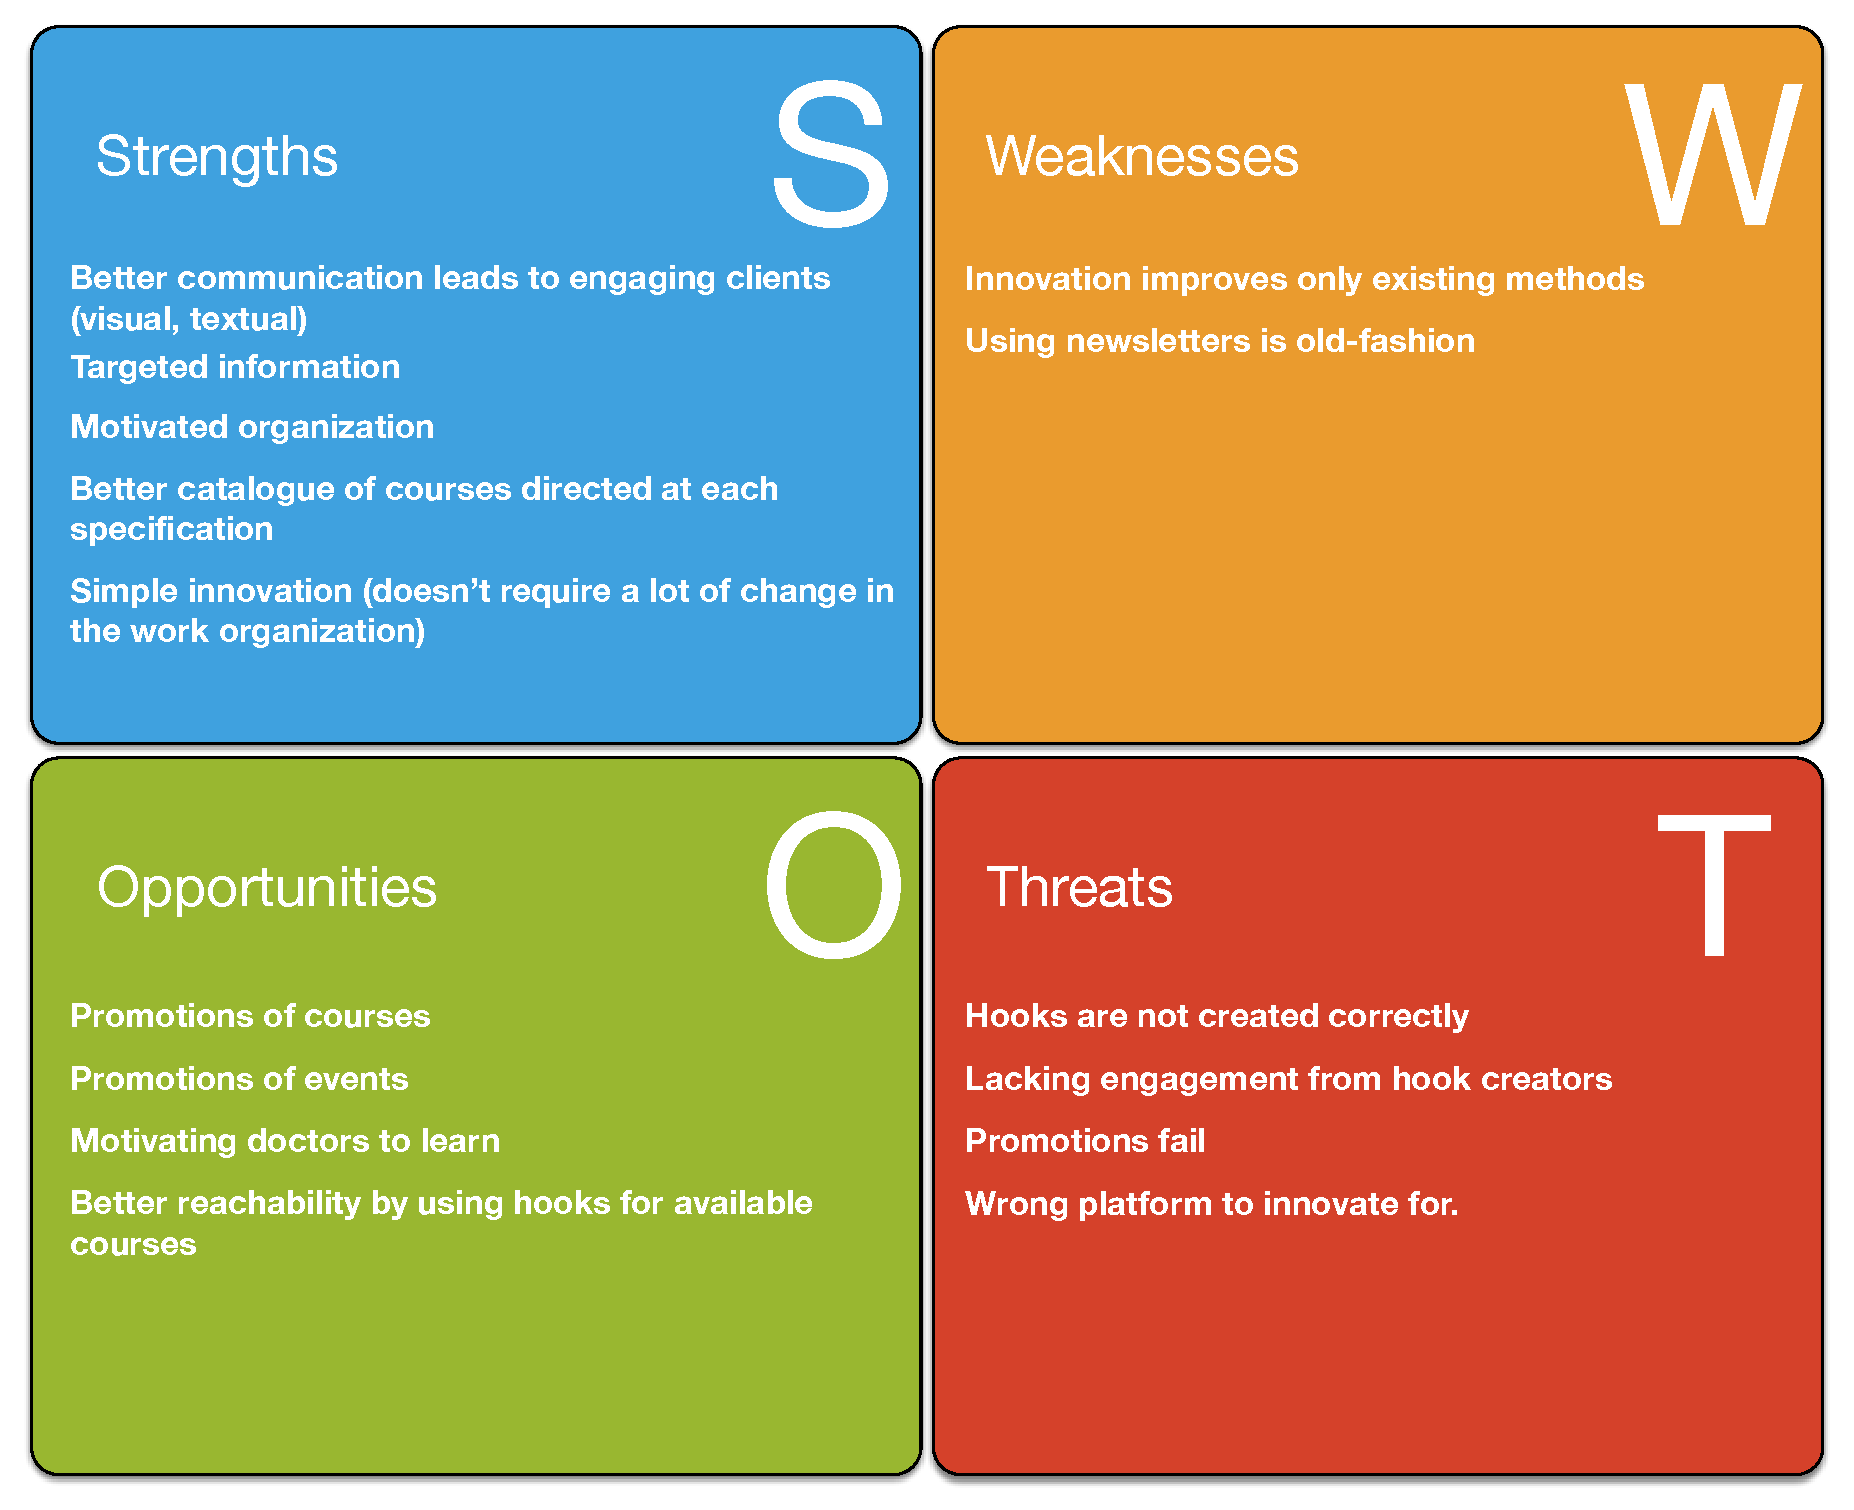
\includegraphics[width=1\textwidth]{figures/swot.pdf}
  \caption{Our baseline-plan for the project.\label{fig:anal_swot}}
 \end{center}
\end{figure*}

\subsection{Finances}
\label{sec:finances}
While this solution does not directly create a new source of income for DMA it does not really come at a great development cost either. The main expense for our innovation would be a content moderator, which DMA already employs. Meanwhile the improvements has the potential to generate value for DMA in the following ways:

\begin{itemize}
\item DMA members become increasingly satisfied with the product DMA provides and thus experiencing more value for their membership money.
\item By creating a platform with focus on a cross-channel strategy, promoting possibly both e-learning courses from partners, who are already creating the e-learning courses, such as BMJ among others, alongside traditional seminars and courses held in partnership of or by DMA, DMA has a chance to strengthen their position in the market for danish CPD courses making their members depend on them even more as a source of course providers.

This means that when DMA wants to promote their own courses they will be able to access some possibly very strong channels to advertise. This way course creators might come to depend on DMA and their platform to promote their courses, and thus ensuring their strong central position prevailing in the future. Meanwhile the increase of supply in courses available through
\end{itemize}

Given that we have moved from designing a custom e-learning solution for DMA to this promotion platform is also clearly reflected in how our Business Model Canvas for the project has changed, from being a potential source of income to instead simply generating value for DMA as seen between Figure \ref{fig:bmc1} and Figure \ref{fig:bmc2}.


\begin{figure*}[h!]
 \begin{center}
  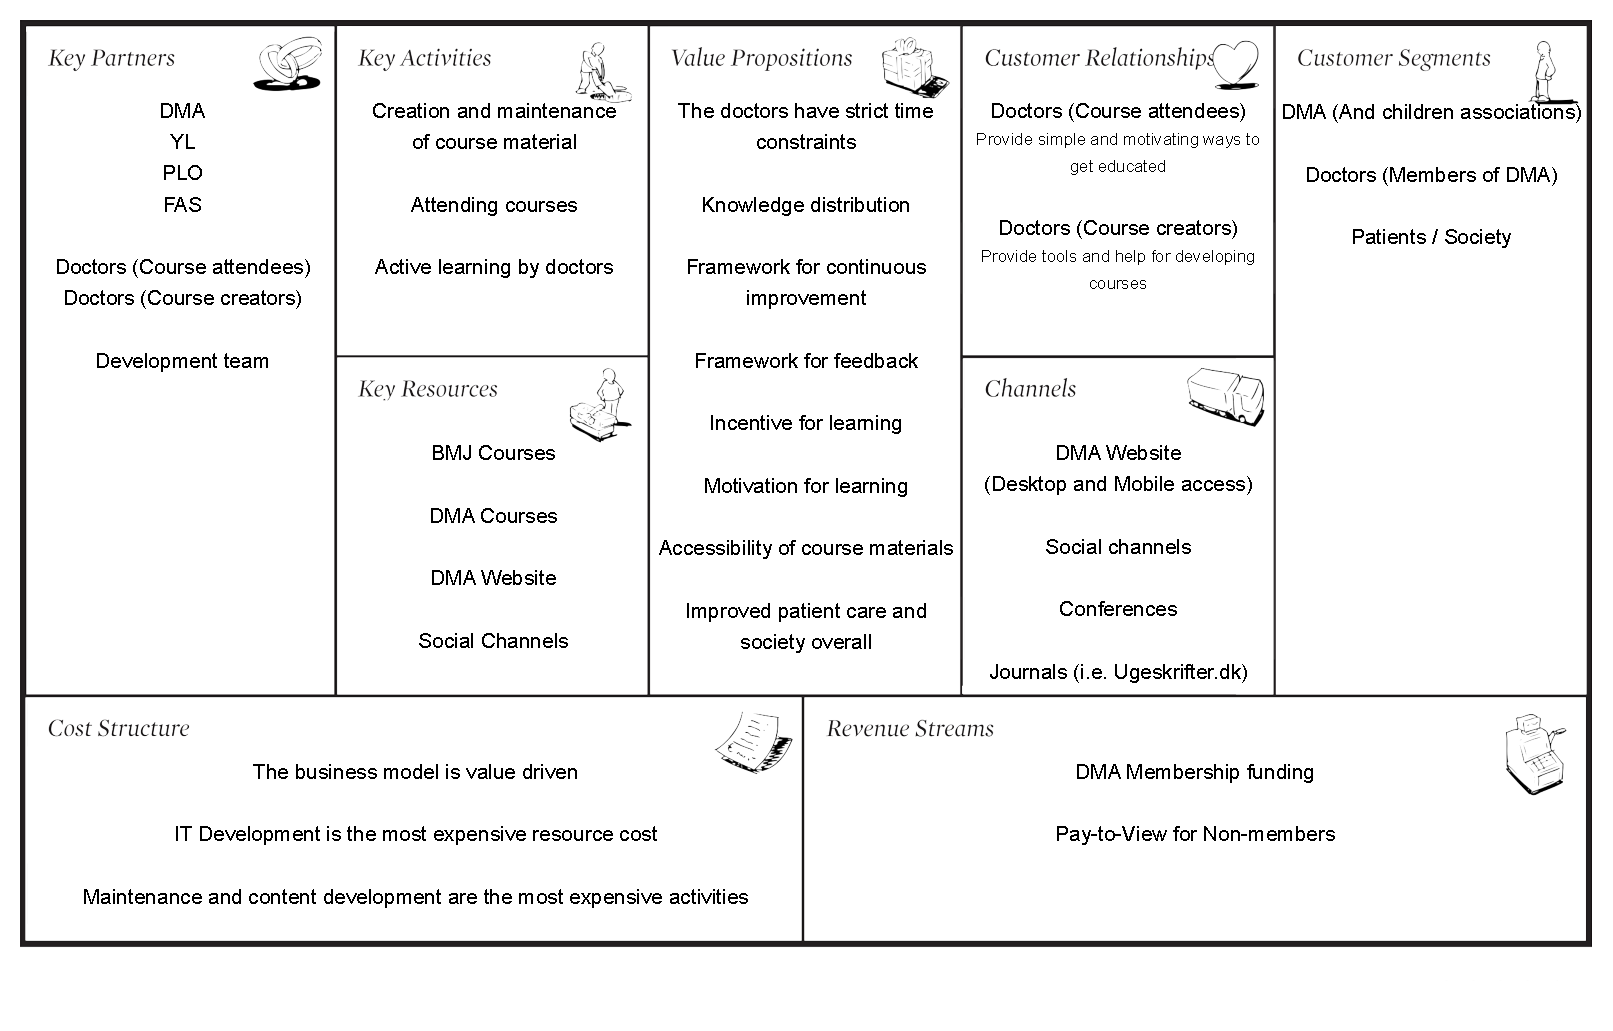
\includegraphics[width=1\textwidth]{figures/Business-Model-Canvas-v1.pdf}
  \caption{The initial BMC analysis for our project.\label{fig:bmc1}}
 \end{center}
\end{figure*}

\begin{figure*}[h!]
 \begin{center}
  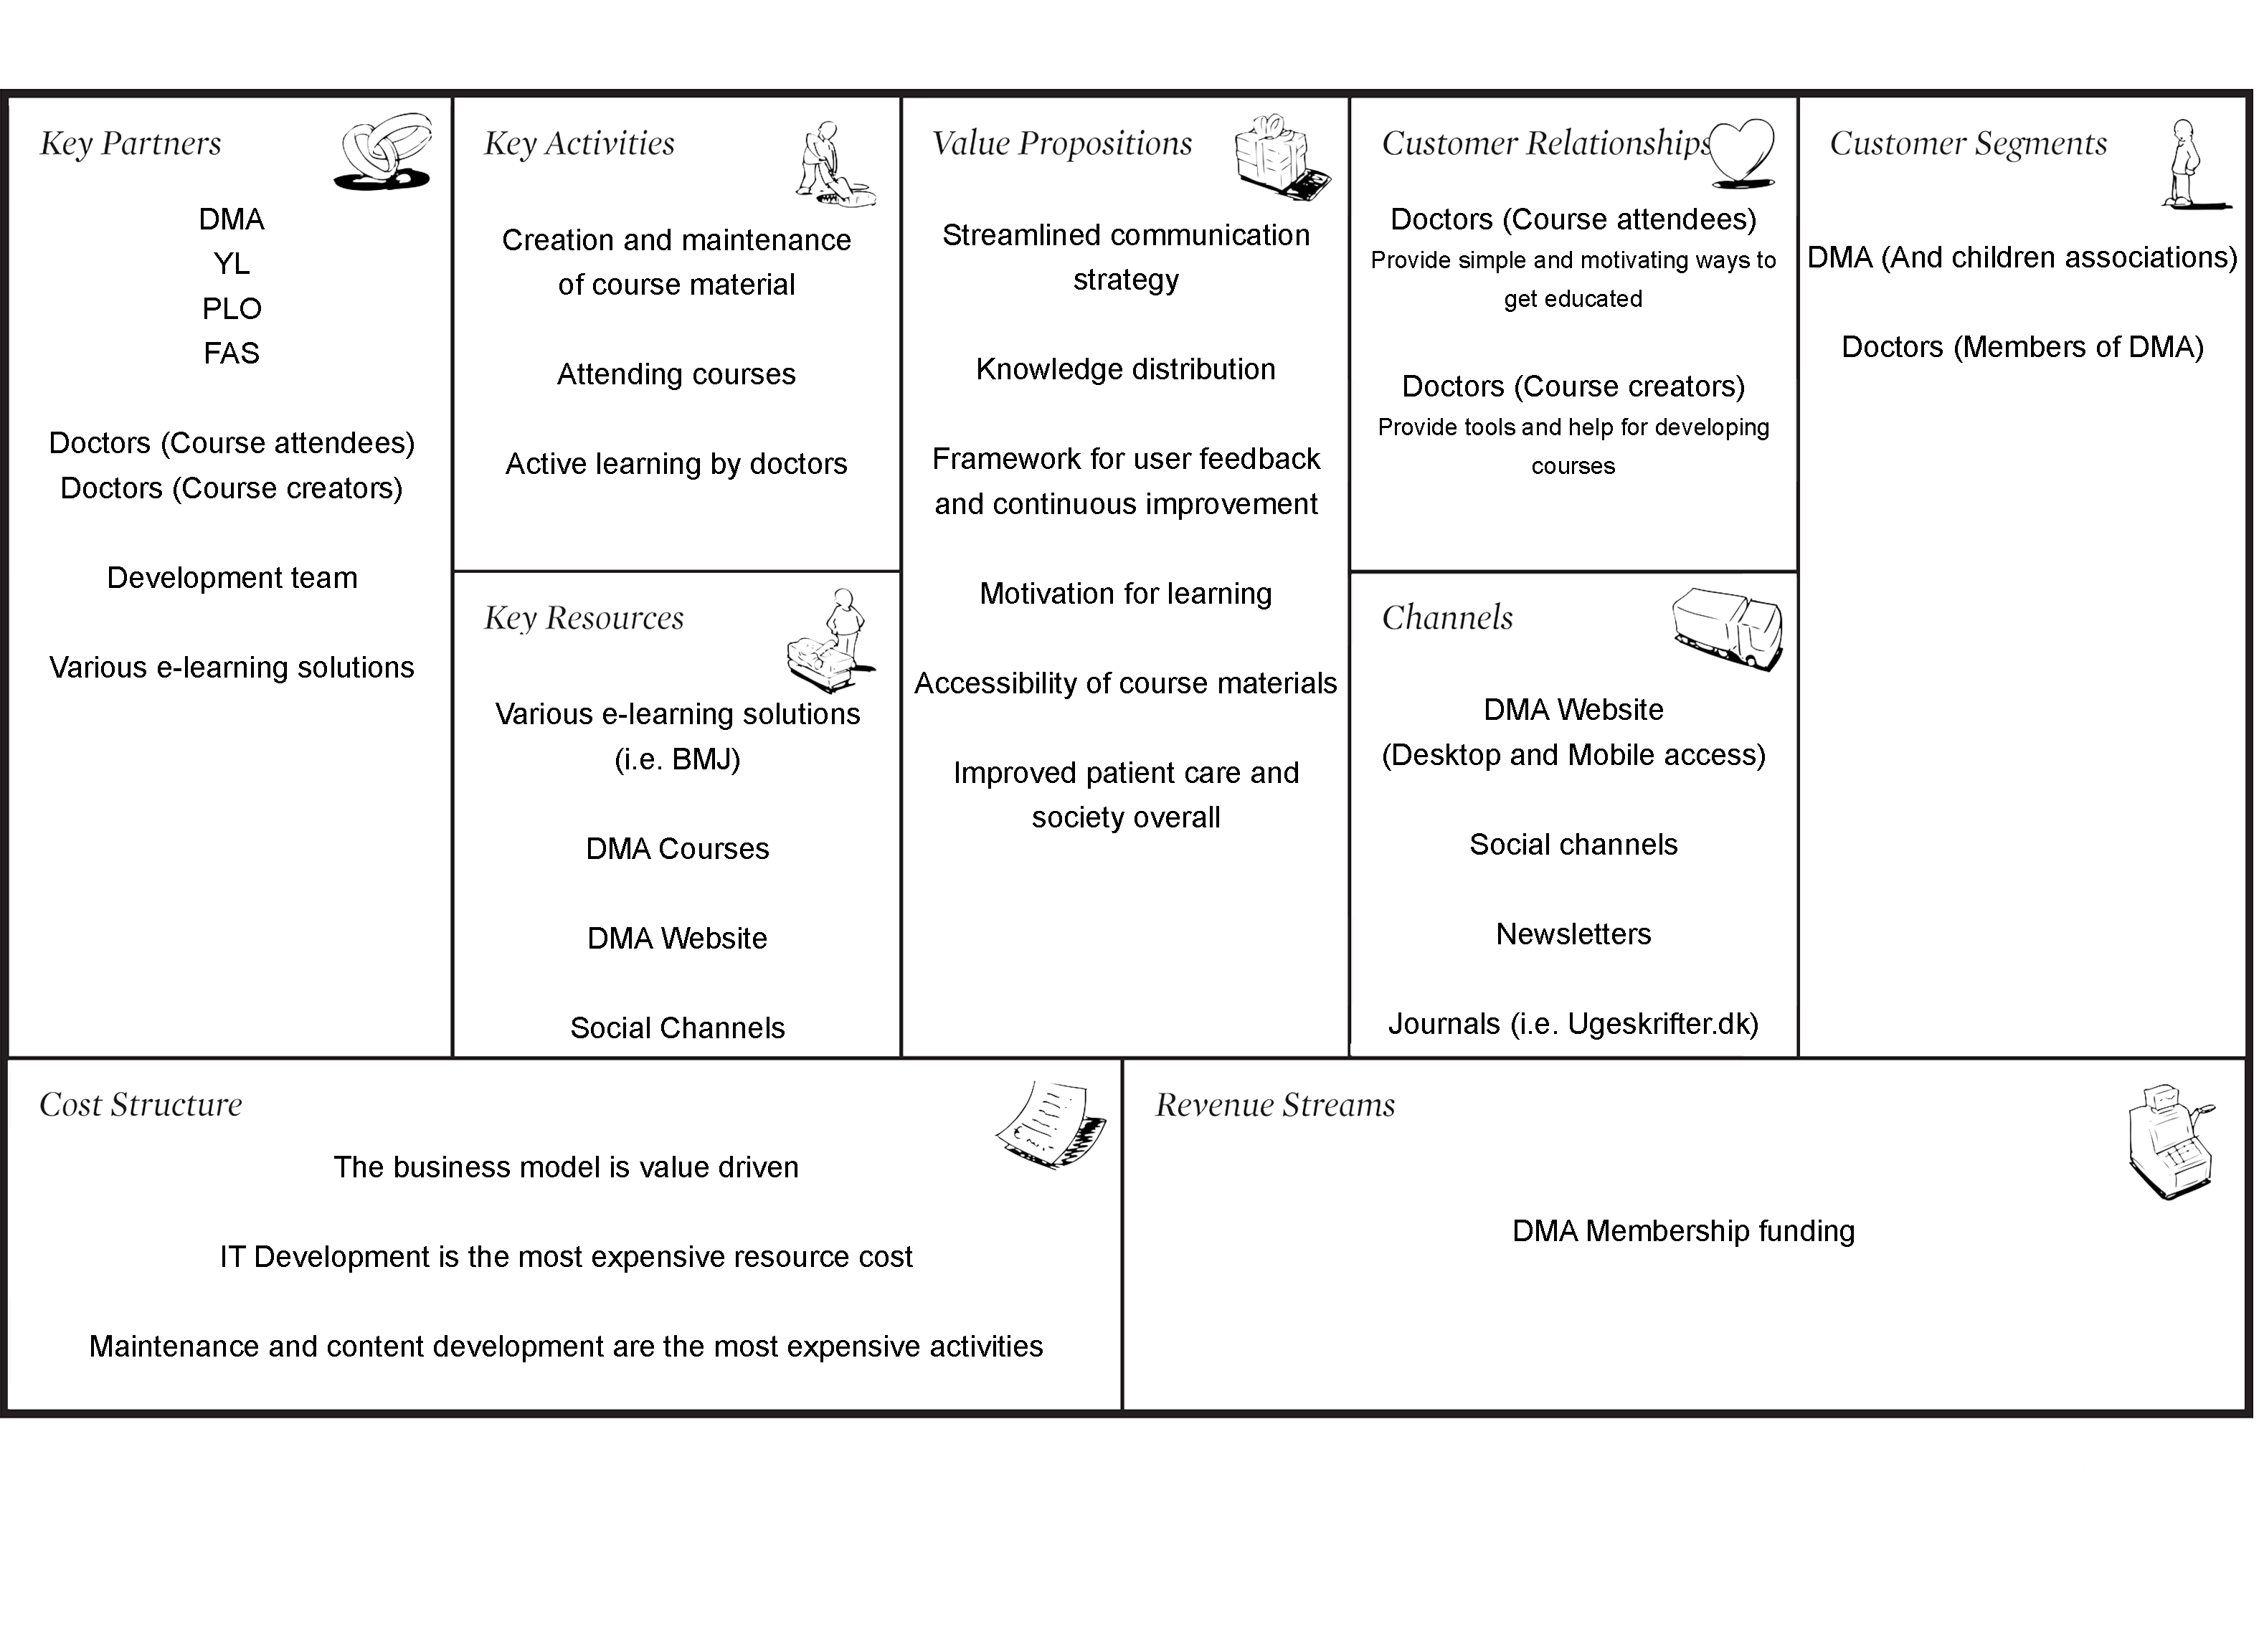
\includegraphics[width=1\textwidth]{figures/Business-Model-Canvas-v2.pdf}
  \caption{The final BMC analysis for our project.\label{fig:bmc2}}
 \end{center}
\end{figure*}

\section{Implementation strategy and plan}
\label{sec:implementation}
The IT systems and IT platform section above explains the situation to some extent, but there are some considerations that we will discuss further here.

DMA is currently in the process of designing their new website, and so the integration of our innovation into their new website needs to be considered. We have been in contact with Claus, the project leader on the new website project, and requested any available resources on the designs of the new website. However, they did not have any such resources available at the time, and so we have been forced to design against an unknown website design. We have therefore designed our mock-ups and innovation approach very generally, so that the “building blocks” we propose can be included in some form or shape regardless of the specifics of the website.

Because we do not have direct access to the new website, we run a risk of the website development team not being able to incorporate our innovation on their current schedule and budget. While not monumental in scope, our additions will need some extra working hours to be incorporated into the new website.

Our innovation of hooking and reeling (section \ref{hookandreel}) can be coated in many different colors. The newsletter version is the very basic version, where a hook in the shape of a video, link to a test or similar is presented along with some very concise basic information about it. This is then simply added to the already existing newsletter. The course page version is the more “advanced” version which is a page on the website with all the same information as the newsletter version but with more information added, such as participant reviews, relevant courses and the likes. If this latter version is implemented, the newsletter version can also simply point to the course page where more information can be found as well as the actual hook.

Whichever solution is used opens up for a wide range of usage possibilities. Once the hook is created and presented in the form of a course page or just a snippet used in the newsletter, this resource can also be presented in any other relevant media. The hook (possibly with a link to the course page) might be presented on relevant Facebook pages, LinkedIn profiles, message boards or any other venue for sharing of information. Thus the innovation is very flexible and can easily be connected to changing circumstances.

\subsection{Technical}
Our solution poses no new technical requirements--every part of the innovation uses already existing solutions, be it the website, newsletter, facebook group, video sharing site (youtube), test hosting site (itslearning) and so on. The only technical needs is then that the upcoming website project gets extended slightly to support the course page and possibly also the course feed. DMA can get by without these by only presenting the hooks in the newsletter and copying the same presentation of the hook on other media, but a central place for these courses in the form of the course pages would boost its effectiveness. All other requirements are already posed by the upcoming website in order for it to be able to function as intended However, keeping our suggested innovation in mind when thinking of the new website could help clarify exactly what is required of the new website platform.

\subsection{Organisational}
The biggest organisational challenge will be deciding who will be responsible for creating, and actually creating, the course hooks. DMA and the course/learning responsible people there would initially do this, but course hooks created by the course source/creator could be preferred.

Once the course hook have been created it needs to be advertised. This requires the hook to be presented with the simple relevant information such as time requirements of the hook, type of the course etc. as described earlier. Once that information has been collected, the hook and information about it needs to be presented in the newspaper as well as other media by which DMA reaches out to the doctors. If the course pages and feeds are implemented, this hook also needs to be added to a course page as well as the website feed. This would be DMA’s responsibility as they are already advertising courses to the doctors through these very same media.

\section{Recommendations and Priorities}
\label{sec:recommendations}
\subsection{Evaluation of Our Suggestions}

Our main suggestion, the course hook in the email newsletter, can in principle immediately be implemented and tested within the current work practices at DMA. More importantly it can be evaluated without much risk or requirements from DMA. There are different ways of evaluating this and we would like to suggest some options:

\subsubsection{A/B Testing of Newsletter}
One way of testing the effect of the course hook is to do an A/B test using the newsletter: Part of the DMA members receive a newsletter with some course recommendations using the existing framework, while another part receives a newsletter where the course hooks are used. The two groups are then compared, fx on how many clicks the course hooks resulted in versus the existing way.

\subsubsection{Hook Comparisons}
We suggest several types of hooks in our solution under the assumption that different things work for different people and this holds true for doctors too. However, it could very well be that some type of hook, for instance an intro video, works exceptionally well, while others are no better or perhaps worse than just having a textual description.

A key part of our suggestion is the importance of clear, concise and specific time annotations on any and all hooks. This is another parameter that should be evaluated, as even though the type of hook might be well chosen, for example a video, if the time needed for it to work is too long. or it’s too short and not comprehensive enough, it may have no effect.

In testing both the type and time aspects of the idea, the A/B testing using the newsletter can be used again. For example to evaluate types a hook of each type could be made for a course with equal time requirements and then the newsletter recipients receive one or the other and the amount of clicks are compared. The hooks could also be sent out together and the recipients would then choose which one to click. It should be noted with this method however, that layout and positioning of the hooks could bring noise to the result.

Similarly, to evaluate time a hook of for example 7 min duration and another of 3 min duration is created and then clicks compared. A/B testing is a good approach for this, as having two of the same type of hook but with different time requirements that the doctor then chooses from, would almost certainly just favour the shortest and perhaps even bring confusion.

\subsection{Success Criteria}
The case description provided by DMA was focused on the creation of a learning platform and service. Our focus has changed to the promotion of courses instead, and this calls for a clear definition of success criteria of our solution. These success criteria should fit with DMA’s overall strategy so it’s possible to gauge whether our solutions helps achieving the goals.

Based on our understanding of the DMA strategy, the initial case description and our work, we have the following suggestions to success criteria:
\begin{description}
\item[More signed up course attendants:] As our suggestions are not strictly tied to e-learning courses but can be applied to any course, one possible criteria could be to simply have more attendants to courses. This can be measured by comparing the number of attendants to courses that DMA does on a yearly basis or by looking at the number of BMJ subscription for example.

\item[More website exposure:] Since the DMA website is a keystone in their strategy, getting more traffic and usage of the site could be a clear goal. DMA already has data on their websites exposure, so tracking that after deploying course hooks and comparing would allow evaluation of this criteria.
\end{description}

\subsection{Risks and Limitations}
Of course, there are many threats to validity regarding our proposed solutions. First of all, given the huge lack of user participation we have not been able to get a feedback on how well the Hook and Reel method works. Ideally we would have loved to create a workshop with a room full of doctors and get a genuine feedback on the use of our prototypes but that is unrealistic and very difficult.

Secondly, there are many things that depend on the quality of the hooks. It is not enough to have actually made the hook, it has to be exciting in some way that really brings out the main points of the course it is representing. Seeing as we suggest that the responsibility of the hook creation should lie in the hands of the course responsible, DMA might not be able to be in full control here.

Thirdly, we are only innovating a small aspect of the whole system. We are not designing or innovating a new platform or coming up with a new way to deliver courses, we are only innovating how it should present them. As younger doctors who are more technologically oriented start to appear and fill the seats of the older generation, the Hook and Reel method might get obsolete.

\subsection{Next step}
Early in our project we identified the doctors work practices and specifically their time constraints as a key issue in making any e-learning approach successful. Although our focus has changed to the work practices at DMA primarily, given more time we would have very much liked to observe doctors, try out our suggestions “in the wild” and generally involve more doctors to establish more intimate knowledge of their work practices.

%\section{Work domains}
We have identified two primary work domains: Course creation and Doctors practice.

\subsection{Course creation}
\subsubsection{Definition}
The course creation work domain is the source that DMA uses to provide material for their members to educate themselves. It is not limited to the creators that DMA are directly linked with, but also external third party creators.

\subsubsection{Characterization}
DMA has multiple sources of courses and material of differing types and they are delivered in different ways, from BMJ’s e-learning platform, DMA’s own courses and courses created elsewhere and communicated to members through and by DMA.

The sources have different delivery methods, course content, evaluation methods and purpose.

DMA primarily uses their website and other IT based channels to inform their members of the existence of these courses, and to some extent also give access to them.

\subsubsection{Discussion/conclusion}
The constraints and methods in course creation are key to determining what is possible to actually do in terms of innovative ideas.

\subsection{Doctors practice}
\subsubsection{Definition}
The actual work practice and daily schedule of DMA’s members, the doctors, and how much time and resources they have available for learning new things. This means both considering the day to day work schedule and any time dedicated to learning.

\subsubsection{Characterization}
Although DMA serves a very diverse member group, there is some common ground and work practices among a large part of their members. The doctors have a busy working day that is not very flexible, making it difficult for them to make time for the current format of provided courses.

Additionally some members lack incentive to prioritise learning over working, as some doctors are paid to learn, others are not.

\subsubsection{Discussion/conclusion}
Whatever the quality of the courses provided by DMA may be, the doctors have to be able to find the time to take them. The courses also need to cater for the actual interests of the doctors and be relevant in their daily work.


%\section{Scope}
The focus of our in-depth analysis phase will be to investigate exactly how the course creation works and what the limitations and possibilities are, and what kind of learning format would actually fit into the doctors’ schedule. The goal is to find out exactly how and where to focus our efforts to help the course creators model their content so the doctors will want to and be able to use it.

We consider our project to be either a situation 3 or 4, as described in Bødker, Kensing & Simonsen (2004), page 142, currently more a 4 than 3. We have limited knowledge of the actual structure of the work domains, and the organization and the amount of interest groups is quite high, putting us in a situation 4. This might change as we narrow our focus though, especially in regards to which course creators we ultimately ending up working with.
We need to gather more data on the work practices in our primary work domains and analyse them to focus our project.

%\section{Business model canvas}
\begin{figure*}
 \begin{center}
  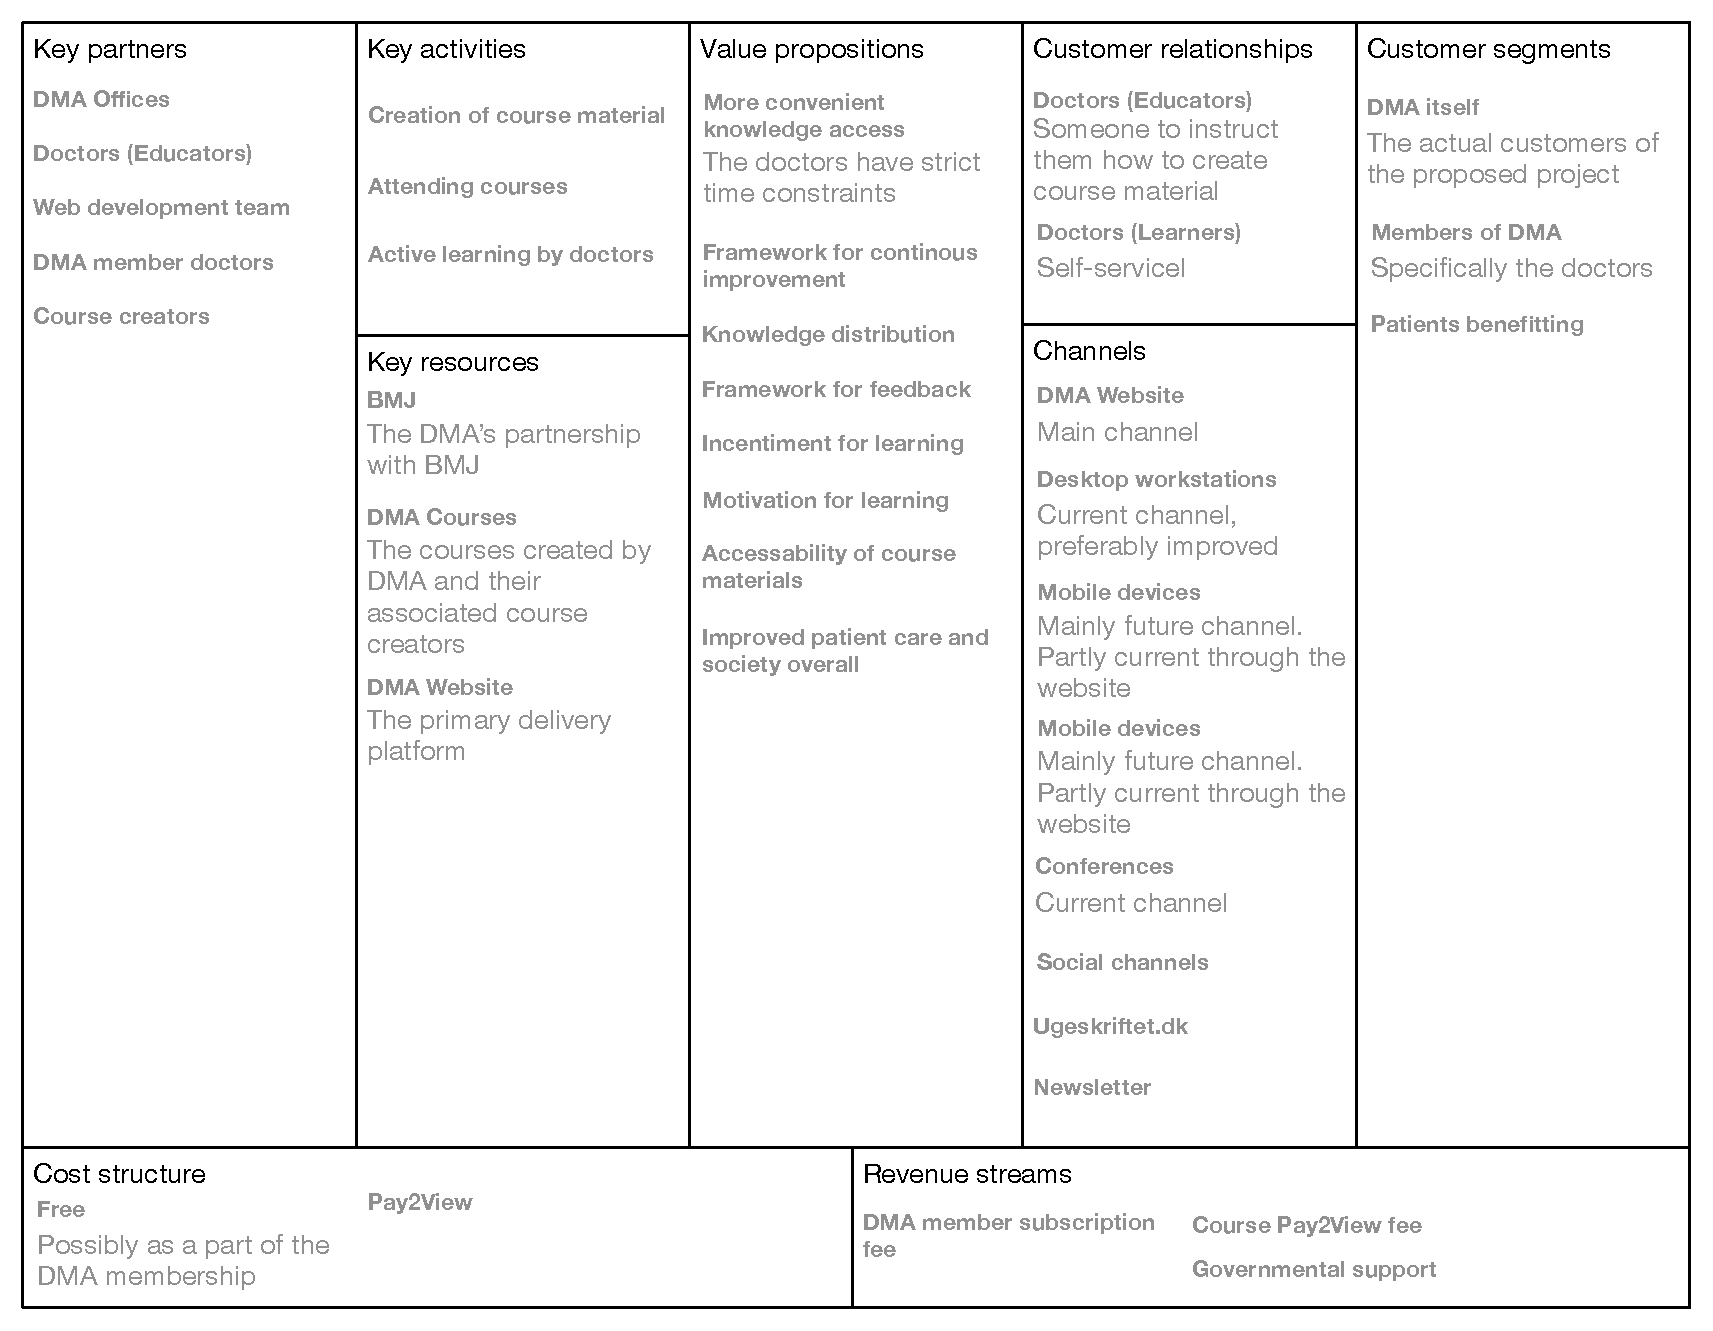
\includegraphics[width=1\textwidth]{figures/business-model-canvas.pdf}
  \caption{Our baseline plan for the project.\label{dmaorganisation}}
 \end{center}
\end{figure*}




\begin{thebibliography}{9}

\bibitem{key-to-success-p1}
  {AKRICH, MADELEINE and CALLON, MICHEL and LATOUR, BRUNO and MONAGHAN, ADRIAN},
  \emph{THE KEY TO SUCCESS IN INNOVATION PART I: THE ART OF INTERESSEMENT},
  International Journal of Innovation Management,
  187-206,
  2002.

\bibitem{key-to-success-p2}
  {AKRICH, MADELEINE and CALLON, MICHEL and LATOUR, BRUNO and MONAGHAN, ADRIAN},
  \emph{THE KEY TO SUCCESS IN INNOVATION PART II: THE ART OF CHOOSING GOOD SPOKESPERSONS},
  International Journal of Innovation Management,
  207-225,
  2002.

\bibitem{bodker}
  {Bodker, Kerl and Kensing, Finn and Simonsen, Jesper},
  \emph{Participatory It Design: Designing for Business and Workplace Realities},
  Cambridge, MA, USA,
  MIT Press,
  2004.

\bibitem{callon}
  {Michel Callon},
  \emph{Some elements of a sociology of translation: domestication of the scallops and the fishermen of St Brieuc Bay},
  The Sociological Review,
  196-233,
  1984.
\end{thebibliography}

\begin{appendices}
\chapter{Questionnaire}\label{appendix:questionnaire}

\section{Aggregated questionnaire answers}

This section is an aggregation of our questionnaire responses of what we learned about the DMA doctors who had participated in the Genetics Course:

\begin{itemize}
    \item They find courses for their continuous professional education through Lægeforeningen. Other resources used are Facebook groups, homepages for societies and colleagues.
    \item They think courses relevant to their interests are easy to find.
    \item They found the DMA Genetics Course very informative and educational (both as new knowledge and as an update on the material).
    \item They are at best working full time, and at worst working much more than that. Days have to be taken out of their schedules to attend courses (and that is in one case planned for).
    \item They prefer physically attending courses to e-learning (although one had had a good experience with a webinar). Other specific forms of learning mentioned were meetings, congress and reading.
    \item They have experienced a couple of e-learning courses but didn’t like them.
    \item One would like for the DMA to develop and offer courses (type not specified). The other isn’t really interested.
    \item They have not tried available e-learning solutions offered such as BMJ and in one case didn’t know they existed.
\end{itemize}

\section{Raw questionnaire answers}

\subsection{Participant One}
\begin{enumerate}
    \item Where or how do you find relevant courses for your continuous professional development?

Via Laegeforeningen.dk or facebook groups

\item Do you think that information about courses relevant to your interests are available and easy to find?
    Yes
\item How did you find the genetics course? What made you take it?

I found it through on Laegeforeningens webside, laegeforeningen.dk. I am currently considering clinical genetics as my medical speciality.

\item What was your overall impression of the genetics course?

    I[t] was informative and educational. I would recommend it.

\item What does your professional weekly schedule look like? Where and how does continuous professional development fit in?

I am currently working 8am to 3:30 pm, so usually I have to take a day off to attend courses.

\item What is your preferred form of learning (i.e. e-learning vs reading books/papers)? In what ways is this method better than other methods you have tried?

I prefer attending courses physically to e-learning.

\item Which e-learning solutions have you had experience with both -- in regards to your continuous professional development and other learning.

During my years studying medicine at Copenhagen University, I have had to take several hand hygiene and fire fighting e-learning courses. They weren't all that great to be honest.

\item Would you like for the DMA to develop and offer courses, e-learning or not, for continued learning?

    Sure. That would be nice.

\item Have you tried available e-learning solutions, such as those provided by BMJ? If not, why have you not tried them?

    No. I did not know they existed.
\end{enumerate}

\subsection{Participant Two}
\begin{enumerate}
    \item Where or how do you find relevant courses for your continuous professional development?

On Lægeforeningen, at homepages for socielties, through colleagues

\item Do you think that information about courses relevant to your interests are available and easy to find?

    Yes

\item How did you find the genetics course? What made you take it?

I found it on the homepage of Lægeforeningen

\item What was your overall impression of the genetics course?

    Very informative and gave me a good update

\item What does your professional weekly schedule look like? Where and how does continuous professional development fit in?

I work often too much, full time in my clinic as GP, 1-2 duties at the out of hour service during a month, and consultant for the national agency for patients complaints and rights

Beside that I'm GP advisor for an international patientorganization

I have an agreement with my colleague to participate in  courses 7-8 days every year

beside that I have the evenings :)

\item What is your preferred form of learning (i.e. e-learning vs reading books/papers)? In what ways is this method better than other methods you have tried?

meetings, congress, and reading

webinar I have tried that once, it was good

\item Which e-learning solutions have you had experience with both -- in regards to your continuous professional development and other learning.

Just tried it a few times, but I dont like it very much

\item Would you like for the DMA to develop and offer courses, e-learning or not, for continued learning?

Not much interest for me

\item Have you tried available e-learning solutions, such as those provided by BMJ? If not, why have you not tried them?

    No. Better like when someone talks about something he/she is really good at, it makes the interest spread to the participants
\end{enumerate}

\subsection{Participant Three}
This was a last minute response. It supports earlier findings, but we did not have time to included in the above questionnaire aggregation:

\begin{enumerate}
    \item Where or how do you find relevant courses for your continuous professional development?

internet \& Medical journals

\item Do you think that information about courses relevant to your interests are available and easy to find?

Yes

\item How did you find the genetics course? What made you take it?

direct Mail from Lægeforeningen

\item What was your overall impression of the genetics course?

Very Good

\item What does your professional weekly schedule look like? Where and how does continuous professional development fit in?

1 night a week otherwise takes time off for courses or conferencs

\item What is your preferred form of learning (i.e. e-learning vs reading books/papers)? In what ways is this method better than other methods you have tried?

reading articles, but e learning helps to get a better overwiev

\item Which e-learning solutions have you had experience with both -- in regards to your continuous professional development and other learning.

Language

\item Would you like for the DMA to develop and offer courses, e-learning or not, for continued learning?

yes

\item Have you tried available e-learning solutions, such as those provided by BMJ? If not, why have you not tried them?

No. Difficult acces


\end{enumerate}

\chapter{Mock-ups}\label{appendix:mockups}

\section{Newsletter}
Figure \ref{fig:newsletter} shows our mock-up of how we envision the course hooks should be presented and featured in the newsletters sent by DMA:

\begin{figure*}[h!]
 \begin{center}
  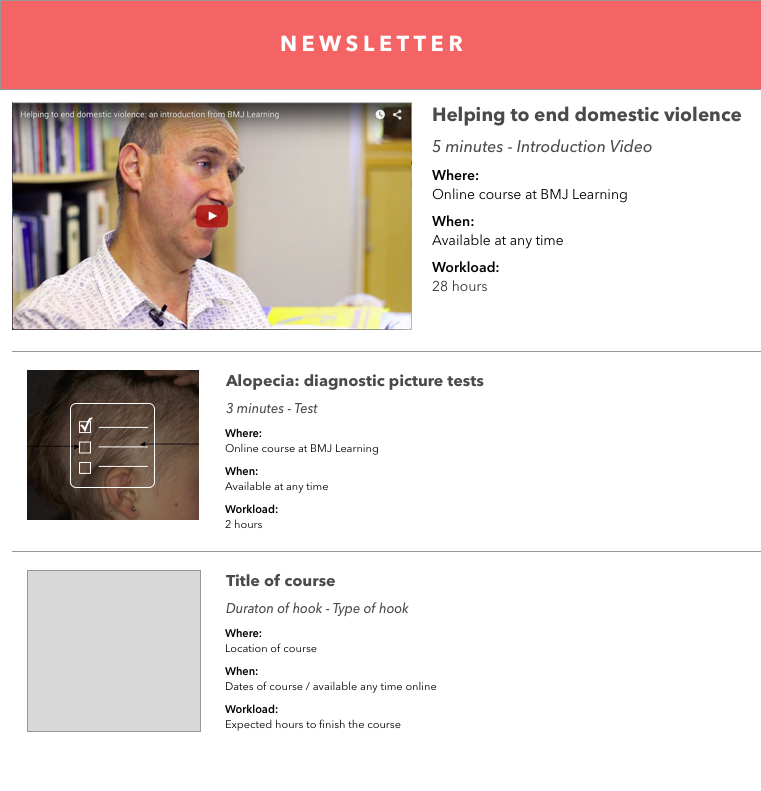
\includegraphics[width=1\textwidth]{figures/newsletter.png}
  \caption{Our mock-up of a newsletter simply presenting the course hooks.\label{fig:newsletter}}
 \end{center}
\end{figure*}

\section{Course page}
Figure \ref{fig:coursepage} shows our mock-up of how we envision the course page on the new DMA website should look, each such page presenting a course hook with additional information such as participant reviews, related courses and what else might be useful:

\begin{figure*}[h!]
 \begin{center}
  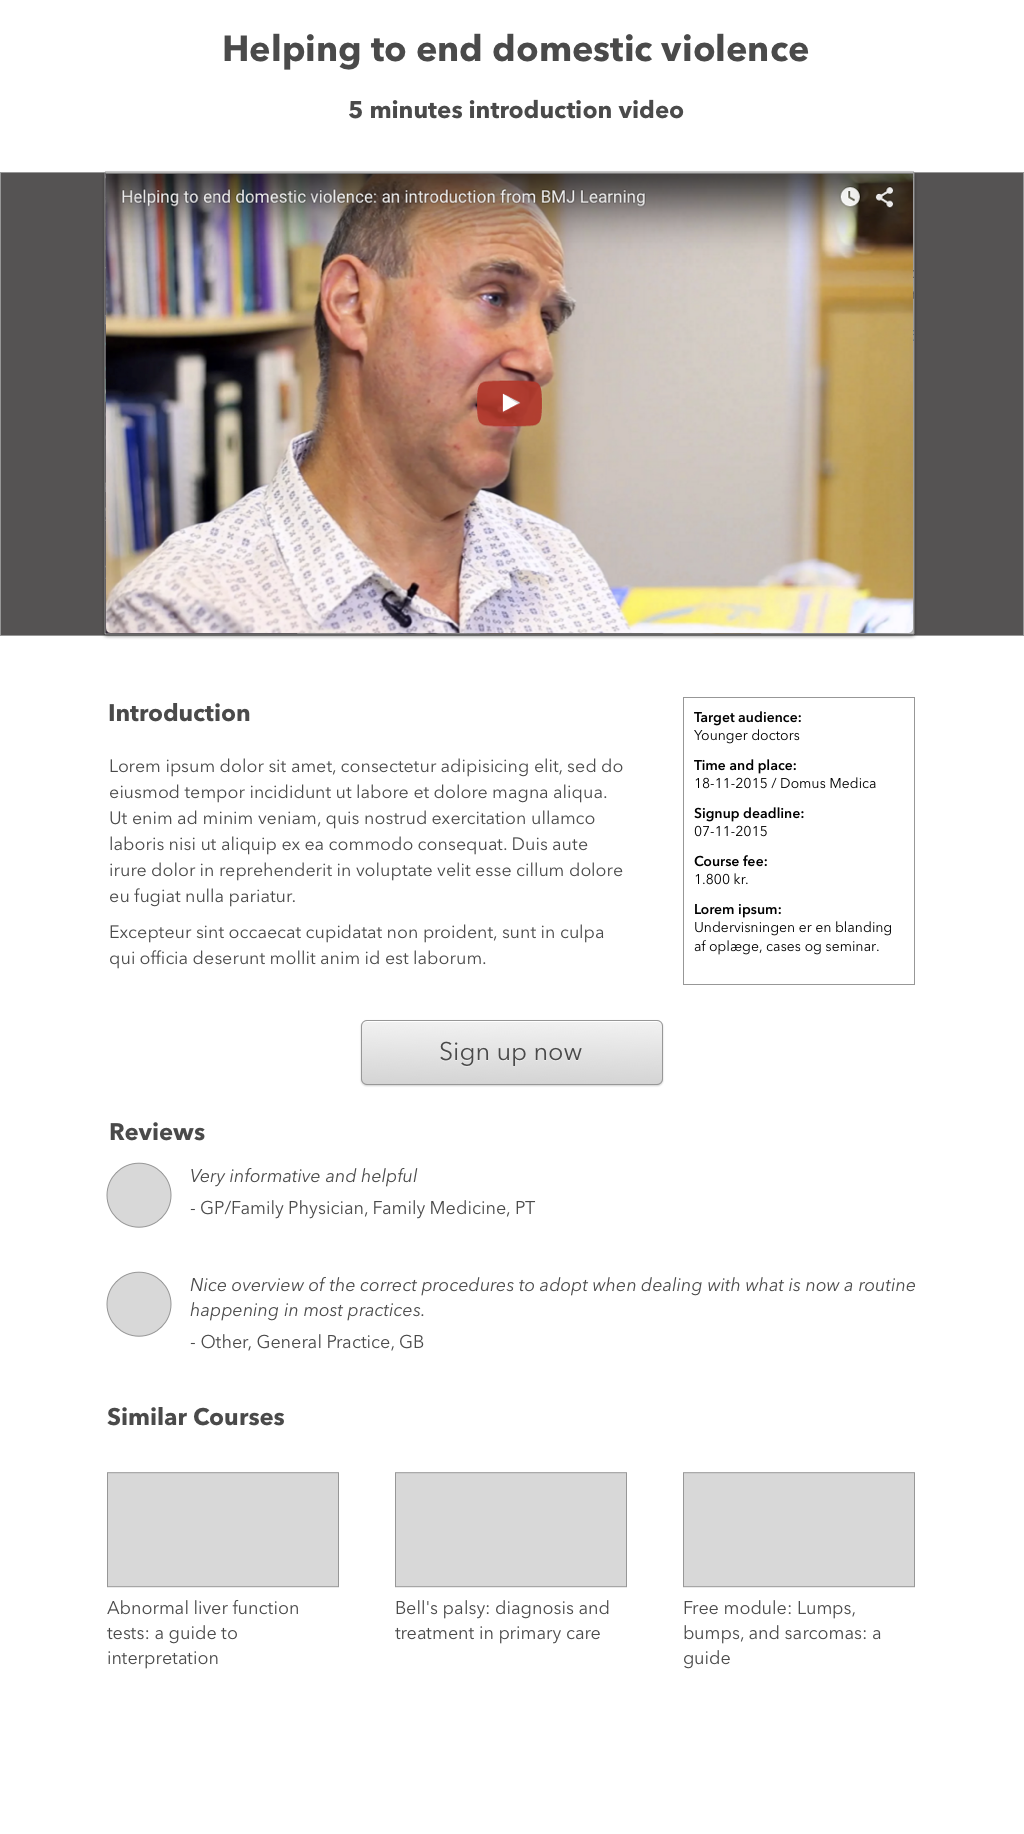
\includegraphics[width=1\textwidth]{figures/coursepage.png}
  \caption{Our mock-up of a course page presenting the course hooks.\label{fig:coursepage}}
 \end{center}
\end{figure*}

\end{appendices}



\end{document}
